
%************************************************
\chapter{Gravitational wave cosmology} \label{chp:gwcosmo}
%************************************************

\begin{flushright}
	\slshape
	I became an astronomer because I could not imagine living on Earth and not trying to understand how the Universe works.\\ \medskip
	--- Vera Rubin
\end{flushright}

In this chapter we want to introduce the field of \ac{GW} cosmology. We start by giving a brief review of the main events that shaped the universe we live in, in section \ref{sec:chronology}. In section \ref{sec:lcdmpuzzles} we then aim at giving a concise overview of the successes the concordance model of cosmology achieved and which unsolved puzzles it leaves us with. \graffito{Outline of this chapter} The following section \ref{sec:homogeneouscosmo} provides a summary of our description of the expansion of space and its effects on the primordial plasma. Section \ref{sec:GWs} then introduces the concept of \acp{GW} in both flat space and a curved background. We will find that \acp{GW} stemming from sources active in the early cosmos are necessarily of stochastic nature today and can leave an observable imprint on the observables of precision cosmology. This chapter will end with a discussion of the existing limits on cosmological \acp{GWB}, stemming from precision cosmology and direct (non-)observations of gravitational radiation. Large parts of this chapter are based on the two famous books by Michele Maggiore~\cite{Maggiore:2007ulw,Maggiore:2018sht} and the detailed review~\cite{Caprini:2018mtu} by Chiara Caprini and Dani Figueroa. The initial sections on the chronology and evolution of our universe on large scales build up on the excellent books by Rocky Kolb and Michael Turner~\cite{Kolb:1990vq}, as well as Daniel Baumann~\cite{Baumann:2022mni}.

\section{Chronology of our universe} \label{sec:chronology}
The best model at our disposal to describe the evolution of the universe is the concordance model. The model can be viewed as a consequence of the two most fundamental theories human minds came up with so far: Albert Einstein's theory of \ac{GR}, describing gravity, and \ac{QFT}, describing all other interactions. The \ac{QFT} that made the mathematical formulation of the concordance model possible is the \acf{SM} of particle physics. In order to make observations fit with theoretical predictions, \graffito{$\Lambda\mathrm{CDM}$} several extensions of the \ac{SM} needed to be introduced, most prominently dark energy ($\Lambda$) and cold dark matter (CDM). These necessary additions to the \ac{SM} give rise to the alternative, more technical name \ac{LCDM} model for the concordance model---and to two yet unsolved mysteries of our universe. The objective of this section is to give a chronological overview of the events which shaped our universe and are described by \ac{LCDM}. A depiction of this timeline can be found in fig.~\ref{fig:timeline}.

\begin{figure}[h]
	\centering
	\begin{tikzpicture}[
		node distance = 2mm and 3mm,
		start chain = A going above,
		dot/.style = {circle, draw=white, very thick, fill=DESYcyan, minimum size=3mm},
		box/.style = {rectangle, text width=50mm, inner xsep=4mm, inner ysep=1mm, font = \small\linespread{0.84}\selectfont, on chain},
		]
		\begin{scope}[every node/.append style={box}]
			\node(1){Today \\ \textcolor{gray}{$t \sim 13.8 \, \text{Gyr}$}};
			\node(2){Recombination \\ \textcolor{gray}{$t \sim 380  \, \text{kyr}$}};
			\node(3){Big Bang Nucleosynthesis\\ \textcolor{gray}{$t \sim 1 \, \text{min}$}};
			\node(4){Electron-positron annihilation\\ \textcolor{gray}{$t \sim 1 \, \text{s}$}};
			\node(5){\acs{QCD} phase transition \\ \textcolor{gray}{$t \sim 20 \, \text{µs}$}};
			\node(6){Electroweak phase transition \\ \textcolor{gray}{$t \sim 10 \, \text{ps}$}};
			\node(7){Inflation};
		\end{scope}
		\draw[very thick, gray, {Circle[length=1pt]}-{Triangle[length=10pt)]},
		shorten <=-3mm, shorten >=-3mm]  
		(A-7.north west) -- (A-1.south west);
		\foreach \i [ count=\j] in {$T\sim240 \, \text{µeV}$, $T\sim250 \, \text{meV}$,  $T\sim100 \, \text{keV}$, $T\sim1 \, \text{MeV}$, $T\sim150 \, \text{MeV}$, $T\sim150 \, \text{GeV}$, ?}
		\node[dot,label=left:\i] at (A-\j.west) {};
	\end{tikzpicture}
	\caption{A timeline of important events in \ac{LCDM} cosmology.}
	\label{fig:timeline}
\end{figure}		

The central observation that made today's theory of cosmology possible is that space expands. Our universe must have hence started in a hot and dense state, which is colloquially referred to as \graffito{The Big Bang} the Big Bang. Due to the mathematical limitations of combining \ac{GR} and \ac{QFT} in a single, agreed-on, more fundamental theory of everything for describing the interactions of matter, only time scales larger than a Planck time ($t_\text{Pl} \simeq 5 \cdot 10^{-44} \, \text{s}$) and length scales larger than a Planck length ($\ell_\text{Pl} \simeq 2 \cdot 10^{-25} \, \text{m}$) can be described reliably. In particular, this forbids any clarifying statements about the initial singularity, which appears if one extrapolates from today's 13.8 billion years old universe back to the state where its energy density exceeded the Planck scale.

The earliest event \ac{LCDM} postulates is cosmic inflation. During this process, which lasted at least $10^{-33} \, \text{s}$, space expanded by a factor of at least $10^{26}$. Inflation \graffito{Inflation} is thought to be triggered by a \ac{PT} of the so-called inflaton field, which also extends the \ac{SM}. Due to the inflaton's high vacuum energy density, space expanded exponentially fast up to the point when the yet cold universe reheated to some temperature below $10^{15} \, \text{GeV}$. During this period of reheating, decays of the inflaton field rapidly filled up the empty space with a thermal bath of SM particles. Due to the strong inflationary period, the plasma is thought to be highly homogeneous, with small inhomogeneities coming from quantum fluctuations of the inflaton field which became macroscopic throughout inflation. These imperfections eventually led to the accumulation of dark matter, acting as a seed for baryonic (``visible'') matter over-densities, which much later evolved into stars, galaxies and larger structures. Additionally, also relic \acp{GW} were produced both through inflation and the subsequent reheating. So far, only the existence of density perturbations with an almost scale-invariant power spectrum has been observed, whereas the \acp{GW} emitted at these early times have not yet been detected~\cite{Planck:2018vyg}.

The next event, which we can be certain occurred, is baryogenesis. During this process, whose precise underlying mechanism is yet unclear, the asymmetry between matter and antimatter has been produced. An often hypothesized connection is with the \ac{EWPT}, happening at temperatures of around $100 \, \text{GeV}$. During this \ac{PT}, the Higgs field of the \ac{SM} obtained its vacuum expectation value, thus giving mass to itself, gauge bosons and fermions. In the \ac{SM}, this \ac{PT} is a cross-over, i.e.~it happens \graffito{The electroweak phase transition} at the same point in time throughout the primordial plasma. There exist several extensions of the \ac{SM} which render the \ac{EWPT} first-order, such that it succeeds through the nucleation of bubbles of the new vacuum state, which then expand, collide and perturb the primordial plasma. Under certain circumstances, the present-day asymmetry between the abundance of matter and antimatter could have been produced in the vicinity of these bubbles~\cite{Baumann:2022mni}. In case the \ac{EWPT} is first-order, \acp{GW} with $\text{mHz}$ frequencies are expected to have been emitted, lying well within the range where the \acf{LISA} will be most sensitive. Hopefully, \ac{LISA} will hence be able to shed light on the mechanism through which the electroweak symmetry was broken in the early universe.

Most particle species of the primordial plasma became massive as a result of the \ac{EWPT}, the only exceptions being photons, gluons and possibly neutrinos remaining massless.\footnote{The \ac{SM} does not allow for the generation of neutrino masses. From the observation of neutrino oscillations we can, however, infer that at least two neutrino families must be massive~\cite{Baumann:2022mni, ParticleDataGroup:2022pth}.} When those massive particles can no longer be produced through thermal processes, because their rest-mass can no longer be reached by the characteristic energy scale of particle interactions set by the decreasing temperature, they typically freeze out of the thermal plasma or become Boltzmann-suppressed. In particular, the thermal freeze-out mechanism is often thought to be the origin of \ac{DM} in our universe, as it naturally gives rise to a \graffito{Freeze-out of \ac{DM}} relic abundance of particles which at most interact  weakly with \ac{SM} particles, matching astrophysical observations. The precise point in time of \ac{DM} freeze-out is a model-dependent question. One of the most studied \ac{DM} candidates, the so-called \ac{WIMP}, is expected to freeze out around the GeV--TeV scale.

The next noteworthy event happening in the early universe plasma is two more \acp{PT} happening at once: Deconfinement and the chiral \ac{PT} are two intertwined \acp{PT} in which quarks and gluons became confined within hadrons, and quarks formed non-zero chiral condensates, respectively. Both events are usually subsumed and referred to as the \ac{QCD} phase \graffito{The QCD phase transition(s)} transition, as in the \ac{SM} they occur simultaneously at a temperature of around $150 \, \text{MeV}$. Both transitions are cross-overs in the \ac{SM}, meaning that the process happens at once throughout the universe and no \acp{GW} are expected to be emitted during the \ac{PT}. There exist extensions of the \ac{SM} which predict one of the two transitions to succeed through the nucleation and expansion of bubbles. The \acp{GW} emitted through this process could have already been observed with \acp{PTA} or be probed in the µHz-band~\cite{Gao:2024pqm}.

Around the MeV scale several events then happened in quick succession: First, neutrinos decoupled from the thermal bath, which was henceforth composed of neutrons, protons, electrons, positrons, photons and a still negligible amount of light nuclei. The neutrinos free-streamed from that point on and only recently became non-relativistic in the late universe. Next, electrons and neutrinos annihilated (up to one part in a billion, due to the previously produced matter-antimatter asymmetry) when the temperature dropped below the electron mass. Their \graffito{$\nu$-decoupling, $e^+e^-$-annihilation and \acs{BBN}} annihilation reheated (or rather: slowed down the cooling of) the remaining bath of nucleons, electrons and photons to a temperature slightly higher than those of neutrinos. Eventually, the nucleons formed (quasi-)stable bound states in a process called \acf{BBN}. The remaining stable bound states are the ionized nuclei of the early elements hydrogen (hydrogen-1 ${}^1\text{H}$ as well as deuterium ${}^2\text{H}$) and helium (${}^3 \text{He}$). To some small fraction also the stable lithium isotope ${}^7 \text{Li}$ has been produced. About three minutes after the end of inflation, the formation of the early elements stalled as the universe had cooled so much that it could no longer sustain nuclear interactions. Today's observations of galaxies with low metallicities in which star formation just started allows us to test the predicted relic abundances of these isotopes observationally. The predictions, being about 75\% hydrogen, 25\% helium and a little ($\mathcal{O}(10^{-10})$) lithium, match the observed mass abundances very well. This success of the \ac{LCDM} model leaves us with the so-called \Neff constraint on new physic at the MeV scale, which we will discuss in section~\ref{sec:BBN}.

Up until 60.000 years after \ac{BBN}, the universe was dominated by relativistic species, commonly referred to as \textit{radiation}. Since the energy density of radiation dilutes faster than that of non-relativistic species, commonly referred to as \textit{matter}, from this point on cold dark and \ac{SM} matter then dominated the cosmic energy budget. In fig.~\ref{fig:earlyuniversediagram} this energy-redshift dependence is plotted. The redshift will be properly defined in the following section, but can intuitively be \graffito{Radiation-Matter equality}understood as the relative factor a wavelength of a photon propagating towards us has been stretched since a given point during cosmic expansion. 

\begin{figure}[t]
	\centering
	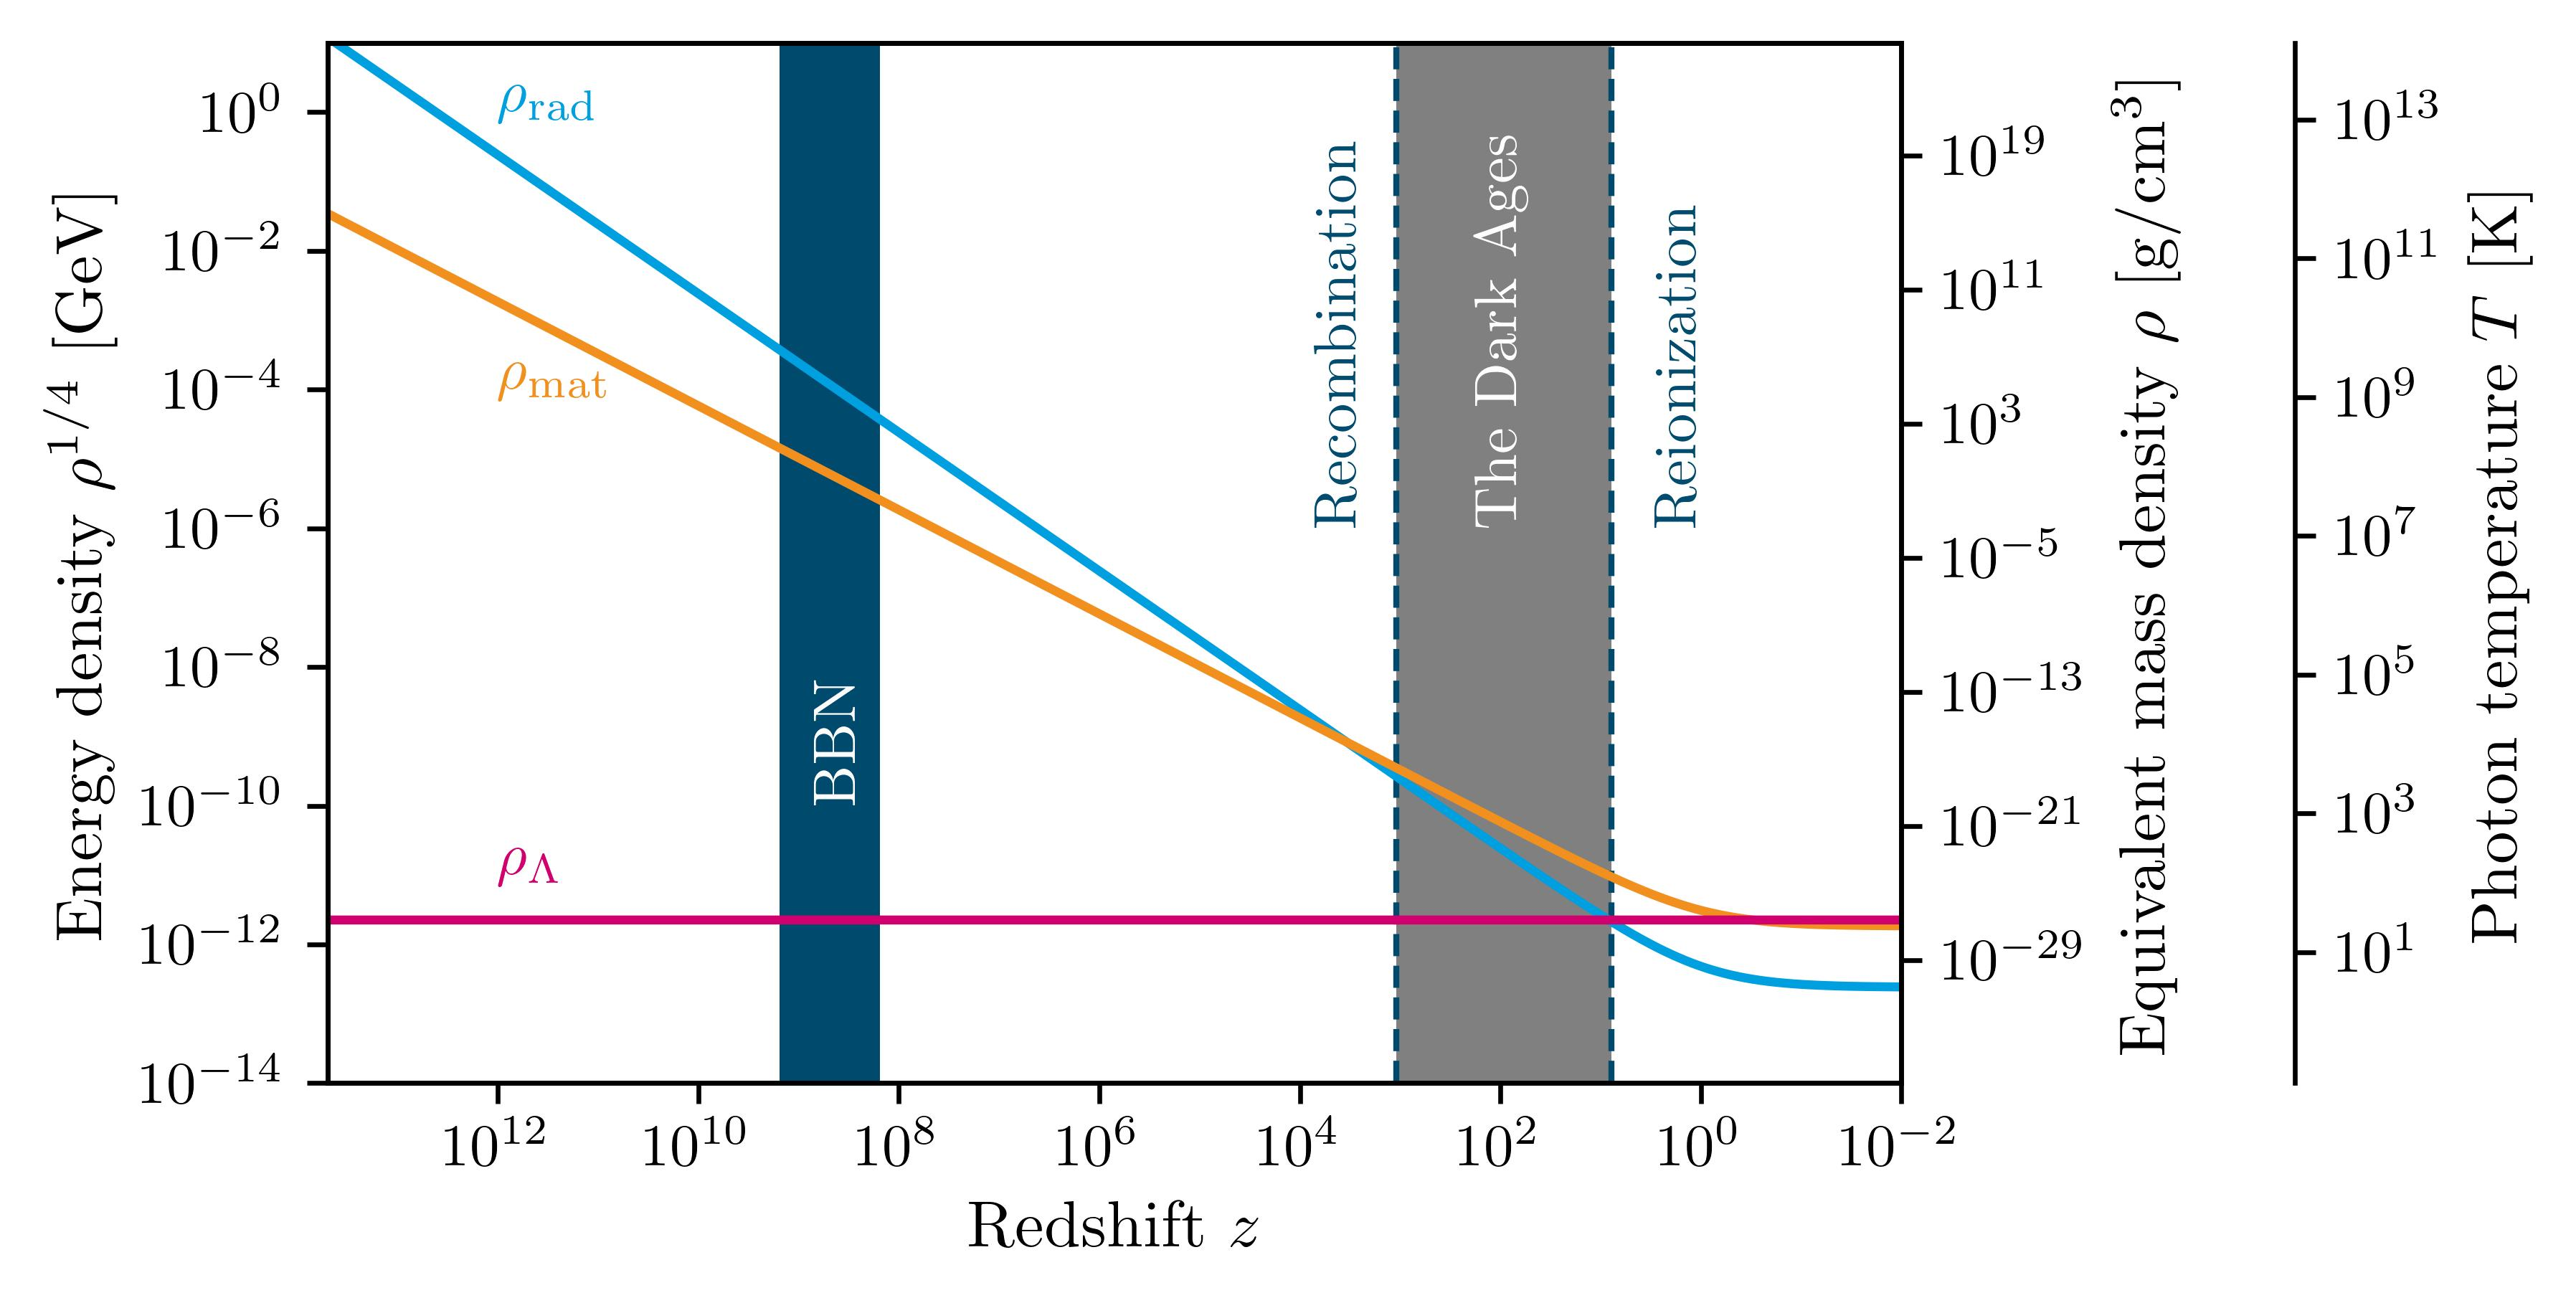
\includegraphics[width=\textwidth]{thesisplots/early_universe_diagram/earlyuniversediagram.jpg}
	\caption{Energy density of the primordial relativistic plasma (rad), the matter energy density (mat) and the vacuum energy density ($\Lambda$) in \ac{LCDM}. The background module of the \texttt{CLASS} code~\cite{Lesgourgues:2011re} and cosmological parameters inferred from Planck 2018 data~\cite{Planck:2018vyg} were used to generate this figure.}
	\label{fig:earlyuniversediagram}
\end{figure}

About 380.000 years after the end of inflation, the universe became transparent to electromagnetic radiation. Whereas it was transparent to \acp{GW} throughout all of the previously discussed processes, photons interacted too frequently with the charged constituents of the plasma for us to still observe them today if emitted before this point in time. Only at recombination, electrons and ionized nuclei formed charge-neutral atoms, allowing photons to free-stream until today.  \graffito{Recombination} The resulting background of photons can be observed today as the \ac{CMB}. The \ac{CMB} can be imagined as an almost perfectly smooth, spherical wall blocking our view towards earlier times.Yet, the \ac{CMB} embodies a rich source of information about the early universe whose interpretation marked the dawn of precision cosmology: after the accidental detection of the \ac{CMB} in 1965 by Penzias and Wilson, the COBE satellite confirmed in 1989 that the \ac{CMB} photons indeed follow an almost perfect black body spectrum with a mean temperature of temperature $2.73 \, \text{K}$ and anisotropies of only one part in 100.000. Subsequent measurements of the \ac{CMB} anisotropies with WMAP and eventually the Planck satellite allowed the formulation of the \ac{LCDM} model. In observing the temperature anisotropies and mapping potential cosmic histories to their angular power spectrum, the age and expansion rate of the universe, as well as its energy composition could be inferred (see fig.~\ref{fig:mattercontenttoday}).

\begin{figure}[t]
	\centering
	\begin{tikzpicture}
		\pie[color={
			DESYcyan30,
			DESYcyan50,
			DESYcyan,
			DESYorange,
			DESYdunkelblau}, radius=2.5, style={ultra thin}]
		{
			5/Baryonic matter,
			26/Dark matter,
			69/Dark energy
		}
	\end{tikzpicture}
	\caption{Today's energy content of the universe, based on the cosmological parameters inferred from Planck 2018 data~\cite{Planck:2018vyg}. The contribution from radiation is $\mathcal{O}(0.1) \, \%$ and was hence neglected in this graphic.}
	\label{fig:mattercontenttoday}
\end{figure}

After the emission of the \ac{CMB}, the universe remained dark for about 10 to 100 million years. The so-called dark ages ended with the cosmic dawn when baryonic matter fell into the potential well of cold \ac{DM}, forming the first (``Population-III'') stars which quickly burned hydrogen and helium to form the first 26 elements of the periodic table. At about the same time reionization \graffito{Reionization} happened: The first stars emitted ionizing photons, thus \textit{re-}ionizing the surrounding gas clouds. Again, the universe became partially opaque due to the scattering of photons with free electrons. Luckily, the ionization was only partial, such that the CMB is not shielded from us, allowing us to still observe it and its anisotropies today.

What follows is the hierarchical structure formation: stars form galaxies, galaxies merged forming bigger galaxies, galaxy clusters, and superclusters, which are separated by large \graffito{Today} voids. Eventually, dark energy dominated over matter, slowing down the formation of larger structures. Recently, life started to evolve somewhere in the Milky Way, which learned how to write PhD theses.

\section{Open questions} \label{sec:lcdmpuzzles}

The \ac{LCDM} model, only being defined through six parameters inferred by observations~\cite{Planck:2018vyg}, is the easiest model able to explain almost all cosmological observables so far. In particular, it precisely explains the power-spectrum of \ac{CMB} anisotropies and the early element abundances produced in \ac{BBN}. It further successfully describes the distribution of galaxies and large-scale structure in our universe, as well as the observed accelerated expansion of our universe. In conclusion, \ac{LCDM} has been remarkably successful in providing a consistent and comprehensive description of our universe, explaining a wide range of seemingly uncorrelated observations like the structure of the \ac{CMB} and galaxy clustering. Yet, there are \graffito{Success and open problems} several pieces of evidence that \ac{LCDM} will not remain the cosmological model preferred by data. The most noteworthy tension today is between local measurements of the current expansion velocity ($\approx 73 \, \text{km}/\text{s}/\text{Mpc}$) and the inferred Hubble rate today from \ac{CMB} data ($\approx 68 \, \text{km}/\text{s}/\text{Mpc}$). Further, there is a mismatch between the predicted and observed abundances of galaxy clusters. The two tensions are referred to as $H_0$ and $\sigma_8$ tension, respectively. To date there is no consensus on how to reconcile those significant tensions in a sole cosmological model which is statistically preferred over \ac{LCDM}~\cite{Schoneberg:2021qvd}. There is, however, serious hope that data from the \ac{JWST} will either help in constructing a new cosmic distance ladder which could either resolve the tensions or provide persuasive evidence for new physics~\cite{Freedman:2023jcz, Freedman:2024eph}.

Further, \ac{LCDM} fundamentally relies on the existence of \ac{DM}, dark energy and an inflaton field, neither of which have been directly observed. The case of \ac{DM} will be of particular importance for this thesis. It therefore makes sense to briefly review the key pieces of evidence for its existence: Cold \ac{DM} is not only motivated through its explanatory power when fitting the \ac{CMB} data to a cosmological model~\cite{Planck:2018vyg}, but further due to several independent sources of evidence: The historically first motivation to introduce this form of non-relativistic (i.e., \textit{cold}) and non-interactive (i.e, \textit{dark}) form of matter was to explain the faster-than-expected movement of galaxies within the Coma cluster by Fritz Zwicky in 1933~\cite{Zwicky:1933gu}. Further evidence for the existence of \ac{DM} was found by Vera Rubin and collaborators in 1970, when they found that observations of galactic rotation \graffito{The evidence for \ac{DM}} curves contradicted expectations based on visible matter only~\cite{Rubin:1970zza}. Whereas these phenomena alone could also be interpreted as a deviation from the Newtonian law of gravity at large distances, several other phenomena motivate the hypothesized existence of \ac{DM}. Studies of galaxy clusters show that the majority of the mass inferred from gravitational lensing is not associated with visible matter~\cite{vanWaerbeke:2000rm, Bacon:2000sy, Wittman:2000tc, Massey:2010hh}. Further, observations of the bullet cluster provide a striking piece of evidence in favor of \ac{DM}: Due to the collision of two galaxy clusters, the distribution of baryonic matter within the bullet cluster, visible as hot gas, differs from the distribution of mass as inferred through gravitational lensing~\cite{Clowe:2006eq, Harvey:2015hha, Robertson:2016qef}. Here, we only listed the key pieces of evidence favoring the existence of dark matter. A thorough review of the mentioned phenomena and other sources of evidence can be found for instance in refs.~\cite{Profumo:2017hqp, Cirelli:2024ssz}.

The shortcoming of the \ac{SM} to provide a viable \ac{DM} candidate motivates the prediction of new particle species, the arguably most famous one being the \ac{WIMP}. By now, the \ac{WIMP} has been subject of many experimental searches, which however only resulted in null-results and exclusion bounds. \graffito{What is \ac{DM} made of?} These, in turn, put the \ac{WIMP} idea under pressure~\cite{Arcadi:2024ukq}. Several other \ac{DM} candidates have been proposed, such as sterile neutrinos, axion-like particles, dark photons, several super-symmetric candidates (such as neutralinos, sneutrinos, gravitinos and axinos), superheavy and composite \ac{DM} particles, as well as \acp{PBH} to just name a few~\cite{Profumo:2017hqp, Cirelli:2024ssz}. 

There has been little progress in settling the debate what \ac{DM} is composed of. This thesis is aimed at contributing to the question how the advent of \ac{GW} cosmology can hopefully shed light on the still mysterious origin of \ac{DM}. In the following sections \ref{sec:homogeneouscosmo} and \ref{sec:GWs} we will start by introducing this new sub-discipline of cosmology. 

\section{The homogeneous universe} \label{sec:homogeneouscosmo}
As introduced above, the evolution of our universe can be derived from coupling Einstein's theory of \ac{GR} with the matter content given by the \ac{SM}. \graffito{Setting the stage for particle cosmology} We will start by solving the Einstein equations for a homogeneous and isotropic perfect fluid and find the Friedmann equations. Those will fix the background evolution and set the stage for the thermodynamic description of the primordial plasma of  elementary particles presented in section~\ref{sec:particlethermodynamics}. In section~\ref{sec:sectors} we will specifically review which impact \ac{DS} particles could have had on the primordial plasma. As cosmology became a mature field over the last decades, the  derivations this abbreviated introduction to cosmology is based on can be found in countless excellent books, see e.g.~\cite{Carroll:2004st, Maggiore:2018sht, Baumann:2022mni}. \acp{GW} and other metric perturbations only played a negligible role throughout the expansion history, such that their impact can be neglected within this section. We will discuss them in the following section~\ref{sec:GWs}.

\subsection{The FLRW metric}

According to \ac{GR}, the gravitational interaction follows the field equations
\begin{align}
	\Mp^2 \, G_{\mu \nu} = T_{\mu \nu} 
	\label{eq:Einstein}
\end{align}
with the Einstein tensor $G_{\mu \nu}$ being a \graffito{The Einstein equations} non-linear function of space-time derivatives of the metric $g_{\mu \nu}$ and the energy-momentum tensor $T_{\mu \nu}$ describing the density and flux of energy and momentum through spacetime. As the cosmological constant $\Lambda$ and the intrinsic curvature of spacetime are irrelevant for the expansion history of the primordial universe, their effect will be ignored in the following discussion.

Observations indicate that our universe is spatially homogeneous and isotropic on large scales. Focussing our discussion on these sufficiently large scales, the metric and the energy-momentum tensor are both subject to tight constraints: Due to homogeneity both quantities can only depend on \graffito{The \acs{FLRW} universe} time, but not on a specific position in space. Isotropy further requires them to be diagonal, where the remaining spatial components are identical. The most general metric that fulfills these criteria for the case of a flat universe is the \ac{FLRW} metric
\begin{align}
	g_{\mu \nu}(t) = \text{diag} \bb{-1, a(t), a(t), a(t)}  .
	\label{eq:FLRWmetric}
\end{align}
The function $a(t)$ is referred to as the scale factor and translates between physical and coordinate distances. It is related to the previously mentioned redshift $z$ of photons from a given cosmic epoch through $a_0 / a = 1 + z$, where $a_0$ is today's scale factor, which is conveniently set to $a_0 = 1$. The energy-momentum tensor is given by
\begin{align}
	T_{\mu \nu}(t) = \text{diag} \bb{-\rho(t), P(t), P(t), P(t)} ,
	\label{eq:perffluid}
\end{align}
where $\rho$ ($P$) is the energy density (pressure) of the perfect fluid as which the hot plasma of the early universe is described. Inserting these quantities into the Einstein field eqs.~\eqref{eq:Einstein} yields two independent differential equations for the scale\graffito{The Friedmann equations} factor, which are referred to as the first and second Friedmann equation. They can be written as
\begin{align}
	H \equiv \frac{\dot{a}}{a} = \sqrt{\frac{\rho}{3  \Mp^2}} \quad &&\text{and}&& \quad
	\dot{\rho} + 3 H  \ba{\rho + P} = 0 \, .
	\label{eq:Friedmann}
	%\dot{H}(t) + H^2(t) = \frac{\ddot{a}(t)}{a(t)} &= - \frac{\rho(t) + 3 \, P(t)}{6 \, \Mp^2} \; .
\end{align}
The first equation defines the Hubble rate $H(t)$, which works as a measure for the expansion rate of the universe at a given point in time. Today's Hubble rate is commonly referred to as the Hubble constant $H_0$. The above set of equations neatly captures the meaning of Wald's famous quote~\cite{Wald:1984rg}: ``Matter tells space how to curve and space tells matter how to move''. Whereas the first Friedmann equation can be identified with the first statement, the second equation maps to the second statement: The energy density of the primordial plasma makes space expand, which in turn leads to the dilution of the plasma.

In the second Friedmann eq.~\eqref{eq:Friedmann}, not only the energy density, but also the pressure of the primordial plasma enters, making the dimensionless equation of state parameter $w = P / \rho$ the decisive quantity for determining the speed with which any form of energy dilutes. For an equation of state $w \neq -1$, we find that $\rho \propto a^{-3(1 + w)}$, $a \propto t^{2(1+w)/3}$ and $H = 2 (1 + w) / (3t)$ by solving the set of the two Friedmann equations. Of particular importance are the cases $w = \frac{1}{3}$ and $w = 0$, corresponding to a \graffito{Equation of state: a song of fire, ice and dark energy} fluid dominated by relativistic and non-relativistic particles, respectively. More conventionally, these fluids are referred to radiation and matter. In these cases the energy density evolves like $\rho_\text{rad} \propto a^{-4}$ and $\rho_\text{mat} \propto a^{-3}$. The case $w = -1$ corresponds to the case of vacuum energy: If vacuum energy dominates over all other energy sources, as in the present universe, the scale factor increases exponentially with time, as vacuum energy does not get diluted by its own induced Hubble expansion.

The total energy density of our universe today is referred to as $\rho_0 = \rho_{\crit,0} \equiv 3 \Mp^2 H^2_0 \simeq 10^{-26} \, \text{kg} / \text{m}^3$, where the Friedmann equation was used to relate its value to the Hubble constant $H_0$. If today's mean energy density were larger (smaller) than this critical value, \graffito{We live in flatland} but $H_0$ remained the same, a positive (negative) intrinsic curvature of Euclidean space would need to be introduced. Measurements of the Planck satellite are however consistent with our universe being intrinsically flat~\cite{Planck:2018vyg}.

We further introduce the normalized energy density $\Omega_i = \rho_{i,0} / \rho_{\crit,0}$, such that $\sum_i \Omega_i = 1$, where the sum runs over all sources $\rho_i$ contributing to the total energy density $\rho$. The current energy densities in radiation, (dark and visible) matter, and dark energy have been inferred from Planck 2018 data~\cite{Planck:2018vyg} and read $\Omega_\text{rad} = 9 \cdot 10^{-5}$, $\Omega_\text{mat} = 0.31$, and $\Omega_\Lambda = 0.69$, c.f.~fig.~\ref{fig:mattercontenttoday}. In this thesis, the Hubble constant \graffito{Today's universe} $H_0 = 67.7\,\text{km}/\text{s}/\text{Mpc} = 2.1 \cdot 10^{-42} \, \text{GeV}$ (based on \texttt{TT,TE,EE+lowE+lensing+BAO} data) is used~\cite{Planck:2018vyg}. In more conventional units, the inverse Hubble constant reads $H_0^{-1} = 4.4 \, \text{Gpc} = 14.5 \, \text{Gyr}$, providing us with a rough estimate of the size and age of the observable universe, ignoring the redshift dependence of its energy content. Integrating the Friedmann equation with the actual energy content described by the above values for $\Omega_\text{rad}$, $\Omega_\text{mat}$ and $\Omega_\Lambda$ leads to the current age of the universe, $t_0 = 13.8 \, \text{Gyr}$.

\subsection{Thermodynamics of the primordial plasma} \label{sec:particlethermodynamics}

So far we assumed that the energy-momentum tensor on the right-hand side of the Einstein eqs.~\eqref{eq:Einstein} is that \graffito{Particles: the actors on the \acs{FLRW} stage} of a generic perfect fluid, which is only characterized by a time-dependent energy density and pressure. The goal of this section will be to derive those two expressions for the particle content of a given \ac{QFT}, in particular of the \ac{SM} and \ac{DS} extensions of it.

The primordial plasma has high number densities and typically also high interaction rates between the different particle species. It can hence be described using the tools of statistical mechanics. As such, we are not interested in the dynamics of individual particles' motions but instead how their distribution changes over time. The distribution $f_a(\bm{x},\bm{p},t)$ of positions and momenta of a given particle species $a$ at a time $t$ is defined such that in a given spatial volume $\mathcal{V}_x$ in a three-dimensional momentum range $\mathcal{V}_p$, the number of particles is defined as
\begin{align}
	N_a(t) = \frac{g_a}{\ba{2 \pi}^3}\int_{\mathcal{V}_x} \diff^3 x \, \int_{\mathcal{V}_p} \diff^3 p \, f_a(\bm{x},\bm{p}, t)
\end{align}
with $g_a$ being the  \graffito{The Boltzmann equation} internal degrees of freedom of species $a$. We now impose that the statistical distribution $f_a$ fulfills the Boltzmann equation
\begin{align}
	\mathcal{L}\bb{f_a} = \mathcal{C}\bb{f_a, ...} .
	\label{eq:Boltzmann}
\end{align}
The Liouville operator $\mathcal{L}$ on the left-hand side relates the geodesics, given a specific metric tensor $g_\mn$, of individual particles of species $a$ to their full distribution $f_a$. The collision operator $\mathcal{C}$ instead relates the changes in the distribution function $f_a$ with those of all other particle species, indicated by the ellipsis in the above equation. The right-hand side describes particle interactions, i.e.~decays and scatterings of $a$, and can thus be understood as the way \ac{QFT} enters into our description of the early universe. 

For an \ac{FLRW} metric, in which $f_a(\bm{x}, \bm{p},t) = f_a(p,t)$ due to isotropy and homogeneity, the Boltzmann equation reads
\begin{align}
	\partial_t f_a(p,t) - H(t) \, p \, \partial_p f_a(p,t) = \frac{C\bb{f_a, ...}(p,t)}{E_a} \, ,
	\label{eq:BoltzmannFLRW}
\end{align}
where $E_a^2 = m_a^2 + p^2$ is the energy of a single $a$ particle with momentum $p$. In practice, this form of the Boltzmann equation is still too generic to infer the dynamics of observable quantities from it. What is often done, is to compute moments of the above partial differential equation in order to obtain a set of ordinary differential equations.

The most relevant moments of the  \graffito{Thermodynamic quantities} distribution $f_a$ in thermodynamics are the number density, the energy density, the pressure and the entropy density of a given species a.  They can be obtained through 
\begin{subequations}
	\label{eq:nrhoPsdefinition}
	\begin{align}
		n_a(t) &= \frac{g_a}{2 \pi^2} \int_0^\infty p^2  f_a(p,t)  \diff p \, ,
		\label{eq:nfromf} \\
		\rho_a(t) &= \frac{g_a}{2 \pi^2} \int_0^\infty p^2 \sqrt{p^2 + m_a^2} f_a(p,t)   \diff p \, , \label{eq:rhofromf}\\
		P_a(t) &= \frac{1}{3} \frac{g_a}{2 \pi^2} \int_0^\infty \frac{p^2 }{\sqrt{p^2 + m_a^2}} f_a(p,t)  \diff p \quad \text{and}\label{eq:pfromf}\\
		s_a(t) &= - \frac{g_a}{2 \pi^2}  \int_0^\infty p^2 \bb{f_a \log \ba{f_a} \mp \ba{1 \pm f_a} \log \ba{1 \pm f_a}}  \diff p \, . \label{eq:sfromf}
	\end{align}
\end{subequations}
The upper \graffito{Moments of the Boltzmann equation} (lower) signs correspond to a bosonic (fermionic) species $a$. Integrating the Boltzmann equation in order to obtain equations of motion for the above quantities, one finds 
\begin{subequations}
	\label{eq:BoltzmannTower}
	\begin{align}
		&\dot{n}_a + 3 H n_a = \frac{g_a}{2 \pi^2} \int_0^\infty p^2 \, \frac{C\bb{f_a, ...}(p,t)}{\sqrt{p^2 + m_a^2}}  \diff p, \label{eq:nBoltzmann} \\
		&\dot{\rho}_a + 3 H\ba{\rho_a + P_a} = \frac{g_a}{2 \pi^2} \int_0^\infty p^2 \, C\bb{f_a, ...}(p,t)  \diff p \label{eq:rhoBoltzmann}\\
		&\dot{s}_a + 3 H s_a = - \frac{g_a}{2 \pi^2} \int_0^\infty p^2 \,  \frac{C\bb{f_a, ...}(p,t)}{\sqrt{p^2 + m_a^2}} \log \ba{\frac{f_a(p,t)}{1 \pm f_a(p,t)}}   \diff p\label{eq:sBoltzmann} \, .
	\end{align}
\end{subequations}
Note that this set of equations for $\dot{n}_a$, $\dot{\rho}_a$, and $\dot{s}_a$ does not necessarily simplify our way to the original goal of simplifying the full Boltzmann equation. Luckily, often the right-hand side can be approximated or be expressed in terms of the same derived quantities $n_a$, $\rho_a$ and $s_a$, allowing an enormous decrease in complexity of the problem. In the case \graffito{The conservation of particle number, entropy and energy} of no particle interactions, $\mathcal{C} = 0$, one finds that the comoving particle number density $N_a = n_a  a^3 $ and the comoving entropy density $S_a = s_a a^3 $ are conserved. For a pressure-less non-interactive species, one further finds that the comoving energy density $\rho_a a^3$ is conserved. For radiation instead, for which $P_a = \rho_a / 3$, this is not the case. In the latter case, the radiation pressure makes the energy density decrease faster and $\rho_a a^4$ is conserved. The underlying physical process is the redshift of the radiation to less energetic, lower frequencies. 

If there is a non-zero collision term for species $a$, the term $\dot{q}_a \equiv \dot{\rho}_a + 3 H \ba{\rho_a + P_a}$ will act as a heat source or sink for other species. The quantity $\dot{q}_a$ is hence often referred to as a heating rate. Comparing the second Friedmann eq.~\eqref{eq:Friedmann} with the \graffito{Adiabatic expansion} expression for $\dot{q}_a$, we can deduce that the total heating rate $\dot{q} = \sum_a \dot{q}_a = 0$ vanishes, such that the total heat $Q = \text{const}$ in the universe is conserved, where $\dot{Q} = \dot{q} a^3$. The Hubble expansion of the universe can hence be understood as an adiabatic expansion in the sense of thermodynamics, slowly cooling down its constituents.

In the case of frequent interactions, the plasma is thermalized. \graffito{Thermal equilibrium} Frequent interactions here refer to an interaction rate which exceeds the Hubble rate, $H\gg \Gamma$. In this case, the distributions can be shown to follow a thermal Bose-Einstein or Fermi-Dirac distribution, 
\begin{align}
	f_a(p, t) = \bb{\exp \ba{\frac{E_a(p) - \mu_a(t)}{T_a(t)} } \mp 1}^{-1} \label{eq:thermalf}
\end{align}
with $\mu_a(t)$ being the chemical potential of $a$. Depending on the strength of interactions allowed by the underlying \ac{QFT}, the temperature $T_a(t)$ either is specific to the species $a$ or shared between several species. In case $a$ only has frequent self-interactions, but no sufficiently fast interactions with other species, $T_a$ is specific for $a$. In case there are frequent interactions involving also another species $b$, the two species thermalize and obtain a common temperature $T_a = T_b$. For the sake of generality, we will for now assume individual temperatures for all particle species.

Plugging in the thermal distribution~\eqref{eq:thermalf} into eq.~\eqref{eq:sfromf} we recover the relation
\begin{align}
	\dot{S}_a &= a^3(t) \frac{g_a}{2 \pi^2} \int_0^\infty p^2 \diff p \, \frac{C\bb{f_a, ...}(p,t)}{E_a}  \frac{E_a(p)- \mu_a(t)}{T_a(t)}  \\
	&= \frac{\dot{Q}_a(t) - \mu_a(t) \dot{N}_a(t)}{T_a(t)}\,, \label{eq:2ndlawIntegrated}
\end{align}
where we introduced the comoving heating rate $\dot{Q}_a \equiv \dot{q}_a a^3$ for species $a$. This is just the second law of thermodynamics, which hence holds for each individual particle species in a comoving volume. From this we can conclude that  a particle species' entropy is conserved individually, when there is no \graffito{Entropy is conserved individually if $\dot{Q}_a = \dot{N}_a = 0$} heat transfer to other particle species, $\dot{Q}_a = 0$, and if the product $\mu_a \dot{N}_a$ vanishes. The latter can be the case if either the chemical potential $\mu_a= 0$ vanishes or if particle number is conserved, $\dot{N}_a = 0$.

Similarly, we can obtain the corresponding relation for the intrinsic thermodynamic quantities, 
\begin{align}
	s_a(t) = \frac{\rho_a(t) + P_a(t) - \mu_a(t) \, n_a(t)}{T_a(t) } \label{eq:2ndlawDensity} \, ,
\end{align}
when plugging the thermal distribution~\eqref{eq:thermalf} into the definitions of $n_a$, $\rho_a$, $P_a$ and $s_a$ in eqs.~\eqref{eq:nrhoPsdefinition}. We can use this equation to calculate the entropy density of a given particle species in thermal equilibrium.

Under the \graffito{Limits for hot and cold species in thermal equilibrium} assumption, that a species is fully relativistic, meaning that its mass and chemical potential are much smaller than its temperature, $T_a \gg \mu_a, m_a$, we obtain
\begin{subequations}
	\begin{align}
		n_a &= g_a \frac{\zeta(3)}{\pi^2} T_a^3(t) \times \begin{cases}
			1 \quad & \text{for bosons}\\
			\frac{3}{4} \quad &\text{for fermions}
		\end{cases} \label{eq:nrel}  \, ,\\
		\rho_a &= g_a \frac{\pi^2}{30} T_a^4 \times \begin{cases}
			1 \quad & \text{for bosons}\\
			\frac{7}{8} \quad &\text{for fermions}
		\end{cases}  \, , \label{eq:rhorel}\\
		P_a &= \frac{\rho_a}{3} \qquad \text{and} \label{eq:Prel} \\
		s_a & = g_a \frac{2 \pi^2}{45} T_a^4 \times \begin{cases}
			1 \quad & \text{for bosons}\\
			\frac{7}{8	} \quad &\text{for fermions}
		\end{cases} \label{eq:srel}  \, .
	\end{align}
\end{subequations}
If instead the particle species $a$ is non-relativistic, $T_a \ll m_a$, such that $E_a\simeq m_a + p^2 / \ba{2 m_a}$, one obtains
\begin{subequations}
	\begin{align}
		n_a &= g_a \ba{\frac{m_a T_a}{2 \pi}}^{3/2} \exp \bb{\frac{\mu_a- m_a}{T_a}}  \label{eq:nnonrel} \, ,\\
		\rho_a &= \ba{m_a + \frac{3}{2} T_a} n_a   \label{eq:rhononrel} \qquad \text{and}\\
		P_a &= T_a n_a \ll \rho_a \, .  \label{eq:Pnonrel}
	\end{align}
\end{subequations}
We recover the well-known Stefan-Boltzmann $T^4$ scaling of the radiation energy density in eq.~\eqref{eq:rhorel}, as well as the Boltzmann-suppression of a non-relativistic species in eq.~\eqref{eq:nnonrel}, together with the ideal gas law in eq.~\eqref{eq:Pnonrel}. We can further identify eq.~\eqref{eq:rhononrel} with the equipartition theorem $\ev{E_a} = m_x + \frac{3}{2} T_a$, also including the rest-mass energy $m_a$ of a single $a$ particle. Eventually, in the limit of $a$ being thermally decoupled, $\dot{q}_a = 0$, we can also retrieve the scaling $\rho_a \propto a^{-4}$  and $\rho_a \propto a^{-3}$ from eq.~\eqref{eq:rhoBoltzmann} for $a$ being relativistic or non-relativistic, respectively. An individual, decoupled species hence just feels the same Hubble expansion as the whole system of coupled fluids.

Without any further ado, we can now perform a sum over all particle species to obtain an expression for the\graffito{Summing over all species} total energy density, entropy and pressure of the primordial plasma, where each individual constituent particle species is (at least individually) in equilibrium,
\begin{align}
	\rho = \sum_a \rho_a \, , && s = \sum_a s_a \, ,&& P = \sum_a P_a \, .
\end{align}
The quantities $\rho$ and $P$ are those that appeared in the Friedmann eqs.~\eqref{eq:Friedmann}. Comparing the expressions derived for a relativistic and non-relativistic species in eqs.~\eqref{eq:rhorel} and~\eqref{eq:rhononrel}, we can see that the expansion will be dominantly driven by relativistic particle species, i.e.~by those satisfying $m_a \ll T_a$. Particles, whose mass exceeds the temperature $T_a$ will quickly become exponentially suppressed due to the Boltzmann factor in eq.~\eqref{eq:nnonrel}, unless they carry a chemical potential, forbidding them to decay or annihilate to lighter states.

\subsection{Dark and visible sectors} \label{sec:sectors}

So far, we only assumed that all particle species can individually be described by a thermal distribution, with a temperature parameter that can differ between different species. Often, however, two particle species $a$ and $b$ carry a common temperature $T_a = T_b$. This is achieved through sufficiently fast interactions between $a$ and $b$. \graffito{A definition for the visible sector} We will use this condition as a definition of what we consider a \textit{sector} of particles. In particular, we will distinguish \textit{visible sector} from \textit{dark sector} particles. Visible sector particles are understood to be those which interact frequently enough with the \ac{SM} photon to form a thermal bath with them.\footnote{For temperatures above that of the electroweak symmetry breaking, when no gauge boson of electromagnetism was existent yet, the analogous massless gauge boson of the hypercharge $U(1)_Y$ is used in this definition of the visible sector.}  For a given temperature $T$ of the photon, this is the case for all relativistic degrees of freedom of the Standard Model, except for neutrinos below MeV temperatures. We will discuss the case of neutrino decoupling towards the end of this subsection. 

Analogously, we define a \ac{DS} to be a thermal bath with a common temperature $T_\text{d}$ between frequently interacting particles, which however \textit{do not} have any sufficiently fast interactions with \ac{SM} particles. In general, the temperature of the \ac{SM} photon therefore does not coincide \graffito{A definition for \acfp{DS}} with the \ac{DS} temperature, $T \neq T_\text{d}$. Note that this definition made no statements about \ac{DM} residing in the \ac{DS}. In particular it should also be noted that it is possible for a \ac{DS} to start thermalizing with the \ac{SM} bath only at a certain point in cosmic history. This scenario will occur in the model discussed in detail in chapter \ref{chp:LISA}. For simplicity, we will still refer to those particles as \ac{DS} states.

The common temperature $T$ of \ac{SM} states motivates the definition of so-called \textit{effective relativistic bosonic energy and entropy \acp{dof}} (or short and less specific, just \textit{effective \acp{dof}}) $g_*(T)$ and $h_*(T)$, which satisfy
\begin{align}
	\rho(T) = g_*(T) \,  \rho_\text{bos}(T) && \text{and}&& s(T) = h_*(T) \,  s_\text{bos}(T) \, , \label{eq:gstar1}
\end{align}
where $\rho_\text{bos} = \frac{\pi^2}{30} T^4$ and $s_\text{bos} =  \frac{2\pi^2}{45} T^3$  are the energy and entropy density of a single massless degree of freedom at temperature $T$ following a Bose-Einstein distribution with vanishing chemical potential. 

The full expressions for the effective \graffito{Counting effective \acp{dof}} \acp{dof} of a set of species with individual temperatures $T_a$ and intrinsic \acp{dof} $g_a$ read~\cite{Husdal:2016haj}
\begin{subequations}
	\label{eq:gstar2}
	\begin{align}
		g_*(T) & = \sum_a g_a  \, \mathcal{G}(z_a)  \ba{\frac{T_a}{T}}^4 \qquad \text{and}\\ 
		h_*(T)	&=  \sum_a g_a  \,   \mathcal{H}(z_a) \ba{\frac{T_a}{T}}^3  , 
	\end{align}
\end{subequations}
where 
\begin{subequations}
	\begin{align}
		\mathcal{G}(z_a) &= \frac{15}{\pi^4} \int_{z_a}^\infty  \frac{u_a^2 \sqrt{u^2_a - z^2_a}}{\mathrm{e}^{u_a} \pm 1} \diff u_a \qquad \text{and}\\
		\mathcal{H}(z_a) &= \frac{3}{4} \mathcal{G}(z_a) +  \frac{15}{4 \pi^4} \int_{z_a}^\infty  \frac{ \ba{u^2_a - z^2_a}^{3/2}}{\mathrm{e}^{u_a} \pm 1} \diff u_a
	\end{align}
\end{subequations}
with $u_a = \sqrt{m_a^2 + p^2}/T$ and $z_a = m_a /T$. The integrals $\mathcal{G}(z)$ and $\mathcal{H}(z)$ can be evaluated numerically and tabulated for a range of $z$. For small $z \ll 1$ (i.e., $m \ll T$), both functions evaluate to 1 for bosonic species and to $7/8$ for fermionic species, whereas for large $z \gg 1$  (i.e., $m \gg T$), both functions approach zero exponentially fast.  Approximately, the effective degrees of freedom are hence just the sum of internal degrees of freedom of those particles which satisfy $m_a \ll T$ (up to a factor $7/8$ for fermions, see eq.~\eqref{eq:rhorel}).

Note, however, the factors $\ba{T_a / T}^4$ and $\ba{T_a / T}^3$ in eqs.~\eqref{eq:gstar2}. \graffito{The case of two secluded thermal baths} Assuming that all particles either can be thought of as visible sector particles with temperature $T$ or \ac{DS} particles with a distinct temperature $T_\text{d} = \xi T$, we obtain
\begin{subequations}
	\label{eq:gstar3}
	\begin{align}
	g_*(T) = \sum_{a \ \text{visible}} g_a  \, \mathcal{G}(z_a) ~ + &~\xi^4 \sum_{a \ \text{dark}} g_a  \, \mathcal{G}(z_a)  \label{eq:gstar}\\
	h_*(T) = \sum_{a \ \text{visible}} g_a  \, \mathcal{H}(z_a) ~ + &~\xi^3 \sum_{a \ \text{dark}} g_a  \, \mathcal{H}(z_a)  \label{eq:hstar} \; .
	\end{align}
\end{subequations}
If the \ac{DS} is colder (hotter) than the visible sector by a factor $\xi$, its contribution to the total energy density will be reduced (enhanced) by a Stefan-Boltzmann factor $\xi^4$. Analogously, the total entropy density will obtain a contribution that scales with $\xi^3$.

One can make the point that also SM neutrinos constitute a \ac{DS} according to the above definition. As mentioned in section \ref{sec:chronology}, neutrinos decouple\graffito{Neutrino decoupling} from the photon bath at a temperature slightly above an MeV. More quantitatively, this happens when the Hubble rate crosses the electroweak interaction rate $\Gamma_\nu \sim G_\text{F}^2 T^5$ with $G_\text{F} = 1.2 \cdot 10^{-5} \, \text{GeV}^{-2}$ for processes like $\nu_e e^- \rightarrow \nu_e e^-$ or $\nu_e \bar{\nu}_e \rightarrow e^+ e^-$ at $T_{\nu\text{-dec}} = 2 - 3 \, \text{MeV}$.\footnote{\label{ftn:nudec}First, the muon and tau neutrinos decouple at a temperature of $3.1 \, \text{MeV}$, followed by the electron neutrinos at $1.9 \, \text{MeV}$. An accurate calculation as performed in ref.~\cite{Lesgourgues:2013sjj} shows that the decoupling temperature is momentum-dependent. We here cite the temperature at which a neutrino with average momentum given their thermal distribution decouples.} At this point in time, the neutrinos inherit the temperature of the photon bath, approximately retaining their Fermi-Dirac distribution. As they are also far from being non-relativistic ($m_\nu \ll \text{MeV}$), their energy density decreases with $a^{-4}$ and their temperature $T_\nu$ hence decreases with $a^{-1}$. When the photon temperature drops below the electron mass, electrons and positrons annihilate.\footnote{\label{ftn:elposann}Being more precise, the long Boltzmann tail of high photon energies leads to the production process $\gamma \gamma \rightarrow e^+ e^-$ being efficient until $T = 0.3 \, \text{MeV}$~\cite{Maggiore:2018sht}.} By that time the neutrinos can be considered to be fully decoupled. As electrons and positrons can only annihilate into photons then, $e^+e^- \rightarrow \gamma \gamma$, the photon bath cools slower than expected by Hubble expansion alone. This process is referred to as reheating, as eventually, the photons will have a slightly higher temperature than neutrinos.

To compute the temperature of the photon bath compared to that of the decoupled neutrinos, we use that entropy is conserved in the bath of \ac{SM} particles. Before the electron-positron annihilation, \graffito{Electron-positron annihilation} the photon (two polarizations), the electron and positron (each having two helicities) and the three neutrino and three antineutrino families, all share the same temperature $T(a_1)$. Using eq.~\eqref{eq:gstar1}, the entropy of the plasma is hence given by
\begin{align}
	s_1 = \frac{2 \pi^2}{45} T^3(a_1) \bb{2 + \frac{7}{8} (2 + 2 + 2 \cdot 3)} .
\end{align}
After the annihilation, only the two photon helicities and six neutrino \acp{dof} are left, where the latter have a to-be-determined temperature $T_\nu(a_2)$ differing from the photon temperature $T(a_2)$. Again using eq.~\eqref{eq:gstar1}, one finds
\begin{align}
	s_2 = \frac{2 \pi^2}{45} \bb{2 \times T^3(a_2) + \frac{7}{8} \times 6 \times  T_\nu^3(a_2)} .
\end{align}
Using entropy conservation, $s_1 a_1^3 = s_2 a_2^3$, together with the condition that the neutrino temperature drops like $T_\nu \propto 1/a$ as they are a non-interacting, relativistic species, we find that
\begin{align}
	T_\nu(a_2) = \ba{\frac{4}{11}}^{1/3} T(a_2) \, .
\end{align}
Since electrons and protons are (\textit{i}) stable, (\textit{ii}) the lightest \ac{SM} states that have non-zero masses and (\textit{iii}) the only species still present in the primordial plasma, there are no more states that could change the photon temperature and neutrino through the above process known as entropy injection. The ratio $T_\nu / T = \ba{\frac{4}{11}}^{1/3}$ hence remains constant up until the point in the late universe when the neutrinos become non-relativistic.

The energy density carried by \graffito{A first encounter with $N_\mathrm{eff}$} the three neutrino and three anti-neutrino degrees of freedoms at a point in time after the electron-positron annihilation is hence given by  
\begin{align}
	\rho_\nu(T) = 3 \times 2 \times \frac{7}{8} \frac{\pi^2}{30} T_\nu^4 = \Neff^\nu \times \frac{7}{4} \frac{\pi^2}{30}\left(\frac{4}{11}\right)^{4 / 3} T^4 \, . \label{eq:rhonuNeff}
\end{align}
Here, we introduced the effective number of neutrinos $\Neff^\nu$, which is used to take into account deviations from the ratio $T_\nu /T = (4/11)^{1/3}$. Assuming the simplified calculation were exact, $\Neff^\nu = 3$ would hold for three SM neutrino families. Taking into account that (\textit{i}) the neutrino decoupling is not instantaneous (see footnote \ref{ftn:nudec}) such that also neutrinos can be partially reheated through the electron-positron annihilation, (\textit{ii}) that the neutrino distribution function is not a perfect Fermi-Dirac distribution after their decoupling, (\textit{iii}) that neutrinos can oscillate into each other, (\textit{iv}) that electrons and positrons were not completely ultra-relativistic at neutrino decoupling and (\textit{v}) finite-temperature effects changing the electron and photon dispersion relations in the plasma, one instead finds $\Neff^\nu = \Neff^\SM = 3.0440 \pm 0.0002$~\cite{Bennett:2020zkv}. In the following we will often encounter $\Neff$ again when deriving cosmological constraints on different expansion histories.

In table \ref{tab:SM}, the mass spectrum of \ac{SM} states as well as their intrinsic \acp{dof} is listed. Summing up all visible sector states, one obtains $g_\SM(T \gg m_t) = h_\SM(T \gg m_t ) = 106.75$ at \graffito{Effective \acp{dof} of the SM} high temperatures. At low temperatures instead, the effect of photon reheating during the electron-positron annihilation is relevant and one obtains $g_\SM(T \ll T_{\nu\text{-dec}}) = 2 + \frac{7}{8} \times 6 \times \ba{\frac{4}{11}}^{4/3} \approx 3.4$ and $h_\SM(T \ll T_{\nu\text{-dec}}) = 2 + \frac{7}{8} \times 6 \times \ba{\frac{4}{11}} \approx 3.9$.

\begin{table}
	\centering
	\begin{tabular}{ccc|ccc}
		\toprule
		Particle $a$ & $m_a$ & $g_a$ & Particle $a$ & $m_a$ & $g_a$   \\
		\midrule  $u, \bar{u}$ & $2.16 \, \mathrm{MeV}$ & 12 & $e^{ \pm}$ & $0.511 \, \mathrm{MeV}$ & 4  \\
		$d, \bar{d}$ & $4.70\, \mathrm{MeV}$ &  12 & $\mu^{ \pm}$ & $105.7 \,\mathrm{MeV}$ & 4 \\
		$s, \bar{s}$ & $93.5\, \mathrm{MeV}$ & 12  & $\tau^{ \pm}$ & $1.777 \,\mathrm{GeV}$ & 4  \\
		$c, \bar{c}$ & $1.27 \,\mathrm{GeV}$ & 12  & $\nu_1, \bar{\nu}_1$ & $<0.082 \,\mathrm{eV}$ & 2\\
		$b, \bar{b}$ & $4.18\, \mathrm{GeV}$ & 12  & $\nu_2, \bar{\nu}_2$ & $<0.082\, \mathrm{eV}$ & 2\\
		$t, \bar{t}$ & $172.6\,\mathrm{GeV}$ & 12  & $\nu_3, \bar{\nu}_3$ & $<0.082\, \mathrm{eV}$ & 2 \\
		\midrule  $g$ & 0 & 16 &  $h$ & $125\, \mathrm{GeV}$ & 1\\
		$\gamma$ & 0 & 2 &&&\\
		$W^{ \pm}$ & $80.4 \,\mathrm{GeV}$ & 6&&& \\
		$Z^0$ & $91.2 \,\mathrm{GeV}$ & 3&&& \\
		\bottomrule
	\end{tabular}
	\caption{The particle content of the \ac{SM} after the \ac{EWPT}. We quote the masses recommended by the particle data group~\cite{ParticleDataGroup:2022pth} for quarks, charged leptons, gauge bosons and the Higgs boson. The tightest constraint on the sum of neutrino masses $m_\text{tot} < 0.082 \, \text{eV}$ is imposed by a combination of BOSS, eBOSS and \ac{CMB} data~\cite{Brieden:2022lsd}.}
	\label{tab:SM}
\end{table}

In the left panel of fig.~\ref{fig:geffs} the effective degrees of freedom of the \ac{SM} are plotted in dependence of the photon temperature. In particular, the \ac{QCD} \ac{PT} can be nicely identified with the the drop in $g_\text{SM}$ around $T = 150 \, \text{MeV}$. The right panel instead shows the impact on the total effective \acp{dof}  of a minimalistic hot \ac{DS} with $\xi = 3$ times higher temperature, containing a \graffito{Effective \acp{dof} from the dark} scalar with $m_\phi = 10^4 \, \GeV$ and a vector boson with $m_{A^\prime} = 10^6 \, \GeV$. Due to the factors $\xi^3$ and $\xi^4$ in eq.~\eqref{eq:gstar3}, already a minimal extension of the \ac{SM} can have important consequences for the expansion history if $\xi > 1$. Note, however, that for this figure it was assumed that the \ac{DS} keeps a temperature ratio of $\xi = 3$ to the \ac{SM} bath over time and that it is able to dispose of its energy density when the \ac{DS} would become non-relativistic, such that the approximation of thermal equilibrium with vanishing \ac{DS} chemical potentials holds at all times.



\begin{figure}[t]
	\centering
	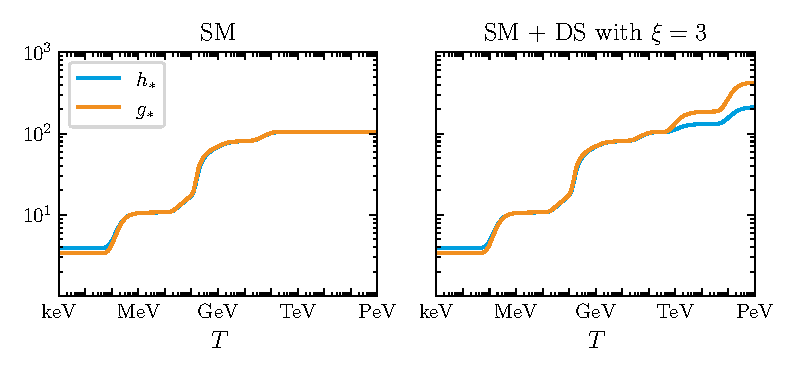
\includegraphics[width=\linewidth]{thesisplots/geff/geffs}
	\caption{Left: Effective \acp{dof} of the \ac{SM} in dependence of temperature. Right: Impact of a hypothetical hot \ac{DS} containing a dark Higgs boson ($m_\phi = 10 \, \text{TeV}$) and a dark photon ($m_A = 1 \, \text{PeV}$) with $\xi = T_\text{d} / T = 3$ on the effective \acp{dof}. To produce this figure, the tabulated data from ref.~\cite{Husdal:2016haj} was used.}
	\label{fig:geffs}
\end{figure}



\subsection{Going out of equilibrium}

Apparently, the usual process of massive particle species becoming more and more Boltzmann-suppressed with decreasing temperatures, up to the point where they become negligible in cosmic history, \graffito{The origin of species} must have exceptions. Otherwise, the energy budget of our universe would only include radiation and vacuum energy today.  Our own existence hence leaves us with a proof that a deviation from equilibrium must have occurred. So far, we have not been very specific in our use of the term equilibrium. Let us introduce the following different types of equilibrium in order to be more precise in the following discussion of what it means for a species to \textit{go out of equilibrium}.

\paragraph{Kinetic equilibrium} refers to a state in which the distribution function $f_a(p,t)$ of a given bosonic (fermionic) species $a$ follows a Bose-Einstein (Fermi-Dirac) distribution~\eqref{eq:thermalf}. It is maintained through self-interactions which redistribute the kinetic energy among particles of the species $a$. Usually, those interactions are elastic scatterings $a a \rightarrow a a$. It implies \graffito{Decoupling = going out of kinetic equilibrium} that the $a$ particles have a common temperature $T_a$. In an extended sense, one can also speak of two species $a$ and $b$ to be in kinetic equilibrium if they share a common temperature $T_a = T_b$. This equilibrium is typically sustained when elastic scatterings $a b \rightarrow a b$ are efficient. The breakdown of the latter equilibrium is referred to as the (kinetic) decoupling of $a$ and $b$.

\paragraph{Chemical equilibrium} is a type of dynamic equilibrium (i.e., all interactions are balanced by their reverse processes, such that the macroscopic properties do not change over time) specific to the particle type. It occurs when there is a balance in particle-type changing interactions, which create and destroy particles of a certain species, such that there is no net change in the number density of that species. \graffito{Freeze-out = going out of chemical equilibrium}  Given two particle species $a$ and $b$ as well as their corresponding antiparticles $\bar{a}$ and $\bar{b}$, chemical equilibrium between $a$ and $b$ is maintained when the interaction rates for $a \bar{a} \leftrightarrow b \bar{b}$ are identical in both directions. For instance, the interaction $e^+ e^- \leftrightarrow \gamma \gamma$  sustained the chemical equilibrium between electrons and photons at high temperatures (c.f., footnote~\ref{ftn:elposann}). More generally, an efficient particle-type changing interaction $ab \leftrightarrow cd$ leads to the species $a$, $b$, $c$ and $d$ to be in chemical equilibrium. If such an interaction ceases to be efficient, the corresponding particles are said to ``freeze out'' since their comoving number densities remain constant in the absence of other interactions.

\paragraph{Thermal equilibrium} is a state between two or more particle species (or in the broader thermodynamic sense: arbitrary subsystems of a total system), which do not have any net energy exchange. This implies that there is a common temperature and no net heat flow between the species in thermal equilibrium. It is maintained if both elastic and particle-type changing interaction between the different particle species are efficient.

Each of these terms usually refers to a specific point in time at which the corresponding interactions which maintain the kind of equilibrium are sufficiently fast. What is meant by \textit{staying in equilibrium} is that the particle interaction rate through which the equilibrium is maintained exceeds the Hubble rate over an extended period of time. Vice versa, when this rate drops below the Hubble rate, the corresponding interactions required to maintain the equilibrium can no longer happen sufficiently fast. Depending on the initial type of equilibrium,  different phenomena can happen: We have already seen at the example of neutrino decoupling what happens when \textit{kinetic} equilibrium (initially sustained by interactions like $\bar{\nu} e^{-} \rightarrow \bar{\nu} e^{-}$) breaks down: there is a decoupling of a species, which will subsequently free-stream. What happens when \textit{chemical} equilibrium breaks down for a species initially in thermal equilibrium with a bath of particles is called the thermal freeze-out\footnote{Technically, also the electron-positron annihilation could be referred to as a freeze-out, given that it starts with a departure from chemical equilibrium. However, in this case the annihilation process $e^+ e^- \rightarrow \gamma \gamma$ only ceases due to the electron chemical potential required by charge neutrality of the bath of electrons and protons and not due to smallness of couplings as in the case of \ac{DM} and neutrons.} and is the subject of the following subsection.

\subsection{The freeze-out of dark matter}

Starting from an initial state in which all particles were in thermal equilibrium with each other, the thermal freeze-out presents a natural way in which a given particle species can escape its fate of disappearing from the thermal plasma due to its Boltzmann-suppression. What needs to happen can \graffito{Chemical potential vs. Boltzmann suppression} already be inferred from the factor $\exp \bb{(\mu - m)/T }$ in eq.~\eqref{eq:nnonrel}: The species needs to develop a non-zero chemical potential which counteracts the Boltzmann-suppression factor $\exp{(-m/T)}$. For this to occur, chemical equilibrium needs to be broken. In other words, the rate of annihilations of that particle species into particles of the thermal bath needs to drop below the Hubble rate in order for the species to \textit{freeze out}.

A particularly well-motivated scenario in which freeze-out produces a relic density of particles is the aforementioned \ac{WIMP} paradigm. Consider a \ac{DM} fermion $\chi$ and its anti-particle $\bar{\chi}$ which can annihilate into an \ac{SM} fermion $\ell$ and its associated anti-particle $\bar{\ell}$. For simplicity we will assume that $\ell$ is essentially massless compared to $\chi$. As $\ell$ is an \ac{SM} particle, it will remain in thermal equilibrium throughout the evolution of $\chi$. Hence, $n_\ell = n_\ell^\text{eq}$ will hold at all times, where $n_\ell^\text{eq}$ \graffito{The Boltzmann equation for DM freeze-out} refers to the number density in eq.~\eqref{eq:nrel}. We will further assume that $\chi$ and $\bar{\chi}$ have equal abundances $n_{\bar{\chi}} = n_\chi$. To be able to use $T \propto a^{-1}$ we will also assume for simplicity, that there are no other annihilations and entropy injections during freeze-out. It can then be shown, that under these conditions the Boltzmann eq.~\eqref{eq:nBoltzmann} for the number density reads (see, e.g.~\cite{Baumann:2022mni, Profumo:2017hqp})
\begin{align}
	\frac{1}{a^3} \td{\ba{n_\chi a^3}}{t} = - \langle \sigma v \rangle \bb{n_\chi^2 - \ba{n_\chi^\text{eq}}^2} \, .
\end{align}
Here, $\langle \sigma v \rangle$ is the thermally averaged\footnote{The averaging refers to an average over relative velocities between $\chi$ and $\bar{\chi}$, on which the cross section $\sigma(v)$ will depend. Given that $\chi$ is in kinetic equilibrium at all times, the distribution of relative velocities can be inferred from the thermal distributions~\eqref{eq:thermalf}.} cross section of the annihilation process. To make the above equation dimensionless in order to solve it numerically, one usually introduces the yield $Y_\chi = n_\chi / s$ and the time parameter $x = m_\chi / T$. One then obtains the Riccati equation
\begin{align}
	\td{Y_\chi}{x} = - \frac{\lambda}{x^2} \bb{Y_\chi^2 - \ba{Y_\chi^\text{eq}}^2} . \label{eq:Riccati}
\end{align}
Here, we further introduced the dimensionless annihilation-rate-to-Hubble-rate ratio $\lambda = \Gamma_\text{ann}(m_\chi) / H(m_\chi)$, where $\Gamma_\text{ann}(T) = \langle \sigma v \rangle n_\chi$ and we assumed $\Gamma_\text{ann}(T) \simeq \Gamma_\text{ann}(m_\chi) $ to be a constant for simplicity. Fig.~\ref{fig:fo} shows numerical solutions to the Riccati equation for a range of interaction rates. One characteristic feature of freeze-out is that it happens at a time $x_\text{f} = \mathcal{O}(10 - 20)$, i.e.~when the number density of $\chi$ is suppressed by $\exp{(-x_\text{f})}$. Moreover, one can see that the yield produced via freeze-out decreases proportionally to $\lambda^{-1}$. \graffito{Analytical solutions} This is due to a later freeze-out in case of a stronger coupling between $\chi$ and $\ell$: The longer $\chi$ stays in chemical equilibrium with $\ell$, the longer its number density can get Boltzmann-suppressed. Ignoring the second term in eq.~\eqref{eq:Riccati}, one can indeed obtain the analytical estimate $Y_\chi^\infty \simeq x_\text{f} / \lambda$ for the relic yield of $\chi$.

\begin{figure}[t]
	\centering
	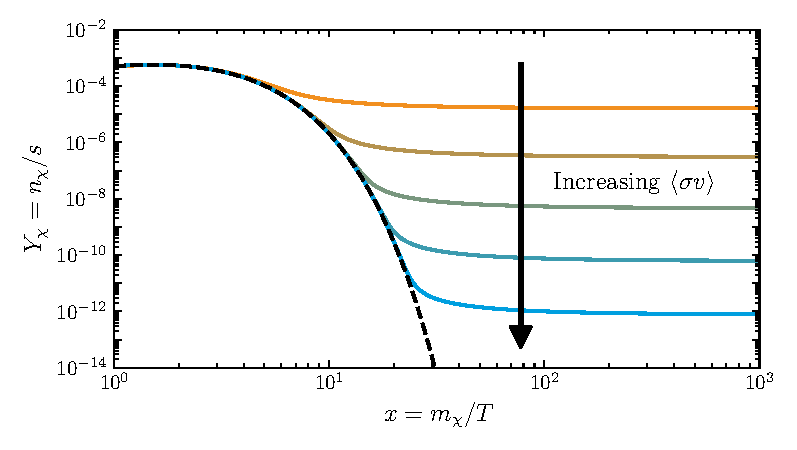
\includegraphics[width=\linewidth]{thesisplots/freezeout/freeze-out}
	\caption{Freeze-out of a scalar $\chi$ with $m_\chi = 1 \, \text{TeV}$ for five thermally averaged cross sections $\langle \sigma v \rangle = 10^{-17} - 10^{-9} \, \text{GeV}^{-2}$ (blue to red curves), each being a factor $10^3$ higher than the previous one. The dashed black line depicts $Y_\chi^\text{eq} = n_\chi^\text{eq}/s$, which $\chi$ would follow if it stayed in chemical equilibrium with the SM bath.}
	\label{fig:fo}
\end{figure}

Using this analytical approximation, one can convert the relic yield $Y_\chi^\infty$ to a relic abundance $\Omega_\chi$ through~\cite{Profumo:2017hqp}
\begin{align}
	\label{eq:FO}
	\Omega_\chi & = \frac{m_\chi}{3\Mp^2 H_0^2} Y_{\chi}^\infty T_0^3 \frac{h_*(T_0)}{h_*(T_\text{f})} \sim 0.1 \frac{x_\text{f}}{\sqrt{g_*(m_\chi)}} \frac{10^{-8} \, \text{GeV}^{-2}}{\langle \sigma v \rangle} \, .
\end{align}
To arrive at this approximate expression for the contribution of $\chi$ to today's matter abundance, we assumed that entropy is conserved between the freeze-out and today, used that $g_*(m_\chi) \simeq h_*(m_\chi)$ as well as $h_*(T_0) = 3.9$, and plugged in the \ac{CMB} temperature $T_0 = 2.7 \, \text{K}$ and the Hubble constant $H_0 = 67.7 \, \text{km}/\text{s} / \text{Mpc}$~\cite{Planck:2018vyg}.

From this analytical estimate we can see that the observed \ac{DM} abundance $\Omega_\DM h^2 = 0.12$ can be produced by a weakly interacting particle with annihilation rates \graffito{The WIMP miracle} into the SM bath of $\sqrt{\langle \sigma v \rangle} \sim 10^{-4} \, \text{GeV}^{-1} \sim 0.1 \, G_\text{F}^{1/2}$. This unexpected coincidence of producing the observed \ac{DM} relic density by a weakly interacting massive particle is usually referred to as the \textit{\ac{WIMP} miracle}.

The thermal freeze-out mechanism can be seen as the starting point of a whole variety of more involved \ac{DM} production mechanisms. An easy extension of the idea is based on the assumption that \ac{DM} never was in thermal equilibrium with the \ac{SM} bath in the first place. This idea led to the discovery of the freeze-in mechanism, which is relevant for \ac{DM} candidates with even lower couplings to the \ac{SM}~\cite{McDonald:1989jd, Hall:2009bx}. \graffito{Variations of the \ac{WIMP} idea} Other noteworthy variations of the \ac{WIMP} idea are for instance based on the assumption of the \ac{DM} mass being lower than that of any \ac{SM} state it can annihilate into (i.e., forbidden \ac{DM}~\cite{Griest:1990kh, DAgnolo:2015ujb}), number-changing processes in the \ac{DS} (i.e., cannibal \ac{DM}~\cite{Dolgov:1980uu, Carlson:1992fn} and pandemic \ac{DM}~\cite{Bringmann:2021tjr}) or a non-\ac{LCDM} expansion history after \ac{DM} production (i.e., homeopathic \ac{DM}~\cite{Cirelli:2018iax, Kamionkowski:1990ni}). An extension of the \ac{WIMP} idea that will be of particular importance for the course of this thesis is the freeze-out of a \ac{WIMP} from a \ac{DS} bath instead of the \ac{SM} bath. This idea will be discussed in chapter~\ref{chp:LISA}.

\subsection{The Big Bang nucleosynthesis} \label{sec:BBN}

In fact, the freeze-out mechanism is not only relevant for the hypothesized production of \ac{WIMP} \ac{DM}, \graffito{Neutron freeze-out sets the initial condition for \ac{BBN}} but also plays a central role within \ac{BBN}. Around the MeV temperature scale, the freeze-out of the processes $n\nu_e \leftrightarrow p^+e^-$ and $n e^+ \leftrightarrow p^+ \bar{\nu}_e$ sets the initial abundance of neutrons, which directly influences the early element abundance produced in \ac{BBN}. 

The chemical equilibrium between protons and neutrons is initially maintained as long as the \graffito{The freeze-out of neutron-proton conversions} rate $\Gamma_{pe\rightarrow n\nu}$ is much larger than the Hubble rate $H(t)$. Ignoring the chemical potentials of electrons and neutrinos, the chemical equilibrium of neutrons and protons implies $\mu_\text{n} = \mu_\text{p}$. Using eq.~\eqref{eq:nnonrel}, the ratio of their number densities hence follows
\begin{align}
	\frac{n_\text{n}}{n_\text{p}} = \ba{\frac{m_\text{n}}{m_\text{p}}}^{3/2} \mathrm{e}^{-(m_\text{n}-m_\text{p})/T} \simeq \mathrm{e}^{-Q/T} \, \label{eq:ntopratio} 
\end{align}
with the mass difference $Q \equiv m_\text{n} - m_\text{p} = 1.30 \, \text{MeV}$. For temperatures above an MeV, neutrons and protons hence have an equivalent number density, whereas for lower temperatures the relative neutron fraction decreases exponentially. If the interactions converting neutrons to protons were infinitely quick, the chemical equilibrium would be maintained and the neutron abundance would have basically vanished before the onset of \ac{BBN} starting with the production of deuterium at $T \lesssim 0.1 \, \text{MeV}$, as we will discuss in more detail below. What happens instead is that the conversion reaction freezes out at $T_\text{f} \simeq 0.8~\text{MeV}$, leaving us with $n_\text{n} / n_\text{p} \simeq 0.20$, i.e. roughly five times more protons than neutrons at that temperature~\cite{Baumann:2022mni}.

A quick estimate of the neutron freeze-out temperature $T_\text{f}$ can be obtained by comparing the rate $\Gamma_\text{weak} \propto G_\text{F}^2 T^5$ for the weak processes  $n\nu_e \rightarrow p^+e^-$ and $n e^+ \rightarrow p^+ \bar{\nu}_e$ with the Hubble rate $H(T)$. Next to the energy density $\rho_\gamma + \rho_\nu$ from photons and neutrinos dominating the cosmic expansion velocity, we also consider an additional energy density $\rho_\text{extra}$ contributing to the Hubble \graffito{The dependence of the neutron freeze-out on $N_\mathrm{eff}$} parameter through the Friedmann eq.~\eqref{eq:Friedmann}.  In eq.~\eqref{eq:rhonuNeff} we introduced the parameter $\Neff^\nu$ to quantify the impact of the number of neutrino species on the temperature ratio between neutrinos and photons after electron-positron annihilation. We now want to parameterize the amount of additional energy density $\rho_\text{extra}$ using the analogous parameter $N_\eff$ defined through
\begin{align}
	\rho_\nu + \rho_\text{extra} \equiv N_\text{eff} \times \frac{7}{8} \ba{\frac{4}{11}}^{4/3} \rho_\gamma \, , 
\end{align}
such that the extra energy can be expressed as\footnote{Note that in general $\DNeff$ is a function of temperature for $\rho_\text{extra}$ having an arbitrary temperature dependence. Only for  $\rho_\text{extra}$ redshifting like radiation $\DNeff$ is a constant.}
\begin{align}
	\rho_\text{extra} = \DNeff \times  \frac{7}{8} \ba{\frac{4}{11}}^{4/3}  \rho_\gamma  \quad \text{where} \quad \DNeff \equiv \Neff - \NeffSM \, . \label{eq:DNeff}
\end{align}
Plugging in $\rho = \rho_\gamma + \rho_\nu + \rho_\text{extra}$ into the first Friedmann eq.~\eqref{eq:Friedmann} to get an expression for $H(T)$ and requiring freeze-out to happen when $\Gamma(T_\text{f}) \simeq H(T_\text{f})$ yields
\begin{align}
	T_\text{f} \simeq \ba{\frac{\pi^2}{45}}^{1/6} \bb{1 + \frac{7}{8} \ba{\frac{4}{11}}^{4/3} \Neff }^{1/6} \frac{1}{\ba{G_\text{F}^2 \Mp}^{1/3}} \, .
\end{align}
For an increase in $\Neff$ with respect to $\NeffSM$, corresponding to a positive contribution $\rho_\text{extra}$ and $\DNeff > 0$, the Hubble expansion is faster, such that the neutron freeze-out occurs at a slightly higher temperature. Due to the exponential sensitivity of the neutron-to-proton ration in eq.~\eqref{eq:ntopratio}, $\Neff$ is hence an important input parameter in any prediction of the early element abundances. In a more \graffito{A faster expansion implies an earlier freeze-out} precise calculation the $\mathcal{O}(1)$ pre-factor and the full temperature dependence of the weak interaction rate, which we here just approximated as $\Gamma_\text{weak} \propto G_\text{F}^2 T^5$, can be determined analytically. Our simplified treatment yields a freeze-out temperature of $1.2 \, \MeV$ for $\Neff = \NeffSM$, which approximately agrees with the previously stated temperature $T_\text{f} = 0.8 \, \MeV$ which results from actually solving the Boltzmann equation, see for instance ref.~\cite{Baumann:2022mni}.

The onset of \ac{BBN} is marked by the formation of deuterium nuclei, composed of one proton and one neutron, as the fusion of two neutrons only leads to a very unstable bound state which immediately decays. Two-proton fusion is also inefficient, as the Coulomb barrier would need to be overcome. Hence, only as soon as deuterium nuclei have formed, more massive elements can form. The deuterium synthesis through \graffito{The onset of BBN: the deuterium bottleneck} the interaction $n + p^+ \rightarrow D^+ + \gamma$ is delayed, however, until a temperature of around $T_\text{D} \simeq 0.1 \, \MeV$ due to the sheer abundance of photons in the plasma. The baryon-to-photon ratio $\eta \equiv n_\gamma / n_\text{b}$ was determined by CMB measurements to be of order $\eta \sim 10^{-9}$~\cite{Planck:2018vyg}, meaning that there are roughly a billion times more photons than neutrons and protons present in the plasma. Due to the long Boltzmann-tail of the photon distribution at high photon energies, the deuterium photo-disintegration only freezes out at a temperature $T_\text{D}$ much lower than the deuterium binding energy $B_\text{D} \equiv m_\text{n} + m_\text{p} - m_\text{B} \simeq 2.22 \, \MeV$. As all other nuclear processes rely on the presence of deuterium due to the above reasoning, this phenomenon became known as the deuterium bottleneck.

Eventually, since the binding energy of helium is larger than that of deuterium, the production rate of helium exceeds that of deuterium. Virtually all neutrons present at the onset of nucleosynthesis will hence end up in ${}^4\text{He}$. The helium mass fraction
\begin{align}
	\mathcal{Y}_p \equiv \frac{4 n_\text{He}}{n_\text{n} +n_\text{p}} = \frac{2 n_\text{n}}{n_\text{n} + n_\text{p}} \simeq 2\left.\frac{ n_\text{n} / n_\text{p}}{1 + n_\text{n} / n_\text{p}}\right|_{\text{D}} \label{eq:Yp}
\end{align}
therefore directly connects the observable relative abundance of ${}^4\text{He}$ \graffito{Virtually all neutrons end up in ${}^4 \text{He}$}  to the neutron-to-proton ratio at the time of the onset of BBN, indicated by a D for the deuterium bottleneck in the above equation. Due to the finite lifetime $\tau_\text{n} = 887 \, \text{s}$ of the neutron, the neutron-to-proton  ratio slightly drops between the neutron freeze-out at $T_\text{f} \simeq 0.8 \, \MeV$ and the formation of deuterium at $T_\text{D} \simeq 0.1 \, \MeV$ from $n_\text{n}/n_\text{p} \simeq 0.20$ to $n_\text{n}/n_\text{p} \simeq 0.14$. Plugging this into the above equation for the helium mass fraction, we obtain $\mathcal{Y}_p = 0.24$, which coincides with the observed value $\mathcal{Y}_p = 0.245 \pm 0.003$. Analogously, one can further set up and solve the Boltzmann equation for the production of heavier elements like deuterium, lithium and beryllium. This task is usually done by tools like \texttt{Primat}~\cite{Pitrou:2019nub} or \texttt{AlterBBN}~\cite{Arbey:2011nf}, which solve the tower of these coupled Boltzmann equations including many hundred nuclear interactions.

In fig.~\ref{fig:bbnsm}, the evolution of the neutron-to-proton ratio (in gray), the helium mass fraction (in blue) and the deuterium fraction (in orange) are depicted. Note how the observed nuclear abundances  \graffito{Precision cosmology} precisely match their predictions. This success of \ac{BBN} to predict nuclear abundances (shown as horizontal dash-dotted lines) up to the percent-level is often referred to by the term precision cosmology.

\begin{figure}[t]
	\centering
	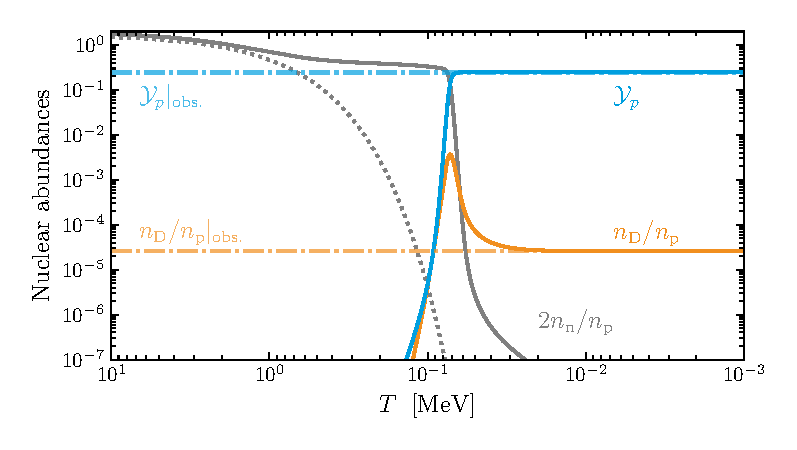
\includegraphics[width=\linewidth]{thesisplots/alteralterbbn_carlo/bbn_sm}
	\caption{Evolution of the neutron-to-proton ratio ({\color{gray}gray}), the helium mass fraction ({\color{DESYcyan}blue}), and the deuterium fraction ({\color{DESYorange}orange}). The equilibrium neutron-to-proton ratio, cf.~eq.~\eqref{eq:ntopratio}, is plotted as a dotted gray line. After the neutron freeze-out at $T_\text{f} \simeq 0.8 \, \text{MeV}$, $n_\text{n}/n_\text{p}$ only decreases slightly due to the neutron decay up to the point when the deuterium photo-disintegration becomes inefficient at $T_\text{D} \simeq 0.1 \, \text{MeV}$. After this point, deuterium can form efficiently and fuse to helium. The data for producing this plot was kindly provided by Frederik Depta.}
	\label{fig:bbnsm}
\end{figure}

Above, we showed that any form of additional energy $\rho_\text{extra}$ results in a larger neutron-to-proton ratio at the time of neutron freeze-out. Due to the above reasoning, this results in an overproduction of ${}^4 \text{He}$. An increase of $\Neff$ by 1 unit (corresponding to the equivalent of one additional neutrino-like species contributing as $\rho_\text{extra}$) would increase the Hubble parameter at that time by $7\%$, leading to a $2\%$ increase in the freeze-out temperature, a $2\%$ increase in the neutron-to-proton ratio and correspondingly also a $2 \%$ increase in $\mathcal{Y}_p$. Since the helium mass fraction was measured on a percent-level, precise bounds on $\Neff$ can be inferred. In our above treatment we have seen, however, that not only $\Neff$, but also the baryon-to-photon ratio $\eta$ is a crucial ingredient in order \graffito{Inferring $N_\mathrm{eff}$ and $\eta$ from BBN} to determine a prediction for the early element abundances.  In a more careful analysis, see~\cite{Baumann:2022mni}, one finds that there is a logarithmic dependence of the predicted helium mass fraction on $\eta$, resulting in a degeneracy between $\Neff$ and $\eta$. This degeneracy can however be resolved when taking into account that the helium fraction is not the only \ac{BBN} observable. In particular, there is a strong dependence of the deuterium fraction $\text{D}/\text{H}$ on $\eta$, leading to a complementary measurement, solving the degeneracy.

Comparing the observations of the early element abundances with their predicted counterparts, one can hence obtain a probability distribution $p(\eta, \Neff)$ which depends on both $\eta$ and $\Neff$. Observational limits on $\Neff$ can then be obtained by combining the distribution $p(\eta, \Neff)$ inferred from \ac{BBN} with its counterpart inferred from \ac{CMB} measurements and marginalizing over $\eta$. Eventually, one obtains the observational bound~\cite{Yeh:2022heq}
\begin{align}
	\Neff = 2.941 \pm 0.143 \label{eq:BBNCMBNeff}
\end{align}
at $95\%$ C.L. We will use this limit on $\Neff$ in two ways in this thesis: The first use will be in constraining the amplitude of cosmological \acp{GWB} in the following section by setting $\rho_\text{extra} = \rho_\gw$ (cf.~eq.~\eqref{eq:NeffboundGW}). In chapter \ref{chp:ptabbn} we will instead interpret $\rho_\text{extra}$ as coming from a \ac{DS}, whose energy is dominated by a plasma reheated in a \ac{PT}.


\section{Cosmological gravitational wave backgrounds}  \label{sec:GWs}

In the previous section \ref{sec:homogeneouscosmo} we discussed the expansion history of our universe. We found that it only depends on the sum of all energy densities and pressure contributions of its individual sub-components, which we described through a perfect, hence spatially homogeneous and isotropic fluid. Obviously, however, the present universe is neither homogeneous nor \graffito{The limits of a perfect fluid description} isotropic---instead its matter distribution is clustered into celestial bodies, galaxies and more extended objects, and large voids. Only when describing large enough scales, the energy distribution and hence the right-hand side of the Einstein eqs.~\eqref{eq:Einstein} can be regarded as being independent of a specific position in space. This section will now try to bridge this gap by considering classes of solutions of the Einstein equation which are not based on the assumptions of statistical homogeneity and isotropy. Instead, we will in particular discuss how \acfp{GW} arise when considering deviations from homogeneity and isotropy.

Historically, the prediction that \ac{GR} features propagating \acp{dof} is almost as old as the theory itself. The derivation was first performed by Albert Einstein himself in 1918~\cite{Einstein:1916cc, Einstein:1918btx}. The existence of \acp{GW} was, however, facing serious doubts for a long time: Sir Arthur Eddington's statement that \acp{GW} would propagate ``at the speed of thought''~\cite{Eddington:1922ds}, \graffito{A short history of doubt} due to some of the wave solutions found by Einstein being gauge artifacts quickly became famous. Together with Nathan Rosen, again even Einstein himself wrote an article in 1936 concluding that \acp{GW} could not exist~\cite{Einstein:1937qu}. The question of the correct gauge choice was only solved two decades later by Felix Pirani in 1956~\cite{Pirani:1956tn}, who showed that passing \acp{GW} could actually move test masses. This idea, eventually led to the ``sticky bead argument'' by Richard Feynman at the first \ac{GR} conference in 1957, which was popularized by Hermann Bondi~\cite{Bondi:1957dt} and convinced physicists at the time that  gravitational radiation is indeed a detectable, physical phenomenon. After some erroneous claims for the observation of \acp{GW} using so-called Weber bars in 1969~\cite{Weber:1969bz}, the first indirect evidence for a \ac{GW}-induced phenomenon came from astrophysics: In 1982, the Hulse-Taylor binary pulsar B1913+16 was shown to have a cumulative shift of its periastron time which precisely followed the prediction of an orbital decay through \ac{GW} emission~\cite{Hulse:1974eb}. Eventually, the first direct detection of \acp{GW} at the \acf{LIGO} in 2014~\cite{LIGOScientific:2016aoc} was made possible through the progress of laser interferometry based on the work of Forward and Weiss in the early 1970s~\cite{Moss:1971ocz, Weiss:2022ols}.

In the following four subsections we introduce the concept of gravitational radiation with increasing levels of diligence: In section \ref{sec:GWinvac} we review the conceptually easiest and \graffito{Outline of this chapter} most well-known scenario of \acp{GW} being the propagating metric perturbations of the linearized Einstein equations. In order to understand the sourcing mechanism of \acp{GW} better we then go over to the more advanced notion of a \ac{GW} as being a gauge-invariant tensor perturbation after performing a helicity decomposition of the Einstein equations into scalar, vector and tensor perturbations around a flat Minkowski metric. This allows us to identify anisotropic stress to be the source of \acp{GW} in section \ref{sec:SVT}. Even after adding this level of complication, there is yet no notion of the energy density of a \ac{GW}. Only after allowing the background metric to back-react on the \ac{GW} by treating it as a dynamical object itself in section~\ref{sec:GWcurvedbackground}, it becomes clear how the energy-momentum tensor of a \ac{GW} can be computed. In section~\ref{sec:GWinFLRW} we finally consider the case that the background through which \acp{GW} propagate is the \ac{FLRW} metric. This brings us straight to the equations of motion of gravitational radiation in the context of cosmology in section \ref{sec:eom}. In section~\ref{sec:stochasticbackgrounds} we then discuss why any \ac{GWB} from the early cosmos can only be detected as a stochastic signal today. Subsections~\ref{sec:spectrum} and \ref{sec:propagation} deal with the different ways a \ac{GW} spectrum can be described and how a cosmic \ac{GWB} gets redshifted until today. Eventually, this chapter concludes with a short review of the bounds on stochastic \acp{GWB} in section \ref{sec:GWlimits}. The main references the following subsections are based on are~\cite{Maggiore:2007ulw, Maggiore:2018sht, Caprini:2018mtu}.

\subsection{Gravitational waves in vacuum} \label{sec:GWinvac}

Let us start with the simplest scenario in which gravitational radiation can be found as a solution of the Einstein eqs.~\eqref{eq:Einstein}. To start with, note that the field equations are by construction invariant under coordinate transformations $x^\mu \rightarrow x^{\prime\mu}(x)$ with $x^{\prime\mu}$ being an arbitrary smooth function of $x^\mu$. To be more precise, $x^{\prime \mu}(x)$ can \graffito{The gauge symmetry of \ac{GR}} be an arbitrary diffeomorphism, i.e.~it has to be invertible, differentiable and its inverse has to be differentiable. Sometimes, this invariance under coordinate transformations is referred to as the gauge symmetry of \ac{GR}. Under these transformations, the metric tensor transforms as
\begin{align}
	g_{\mu \nu}(x) \rightarrow g^\prime_{\mu \nu}\ba{x^\prime} = \pd{x^\rho}{x^{\prime \mu}}\, \pd{x^\sigma}{x^{\prime \nu}} \,g_{\rho \sigma}(x) \, .
	\label{eq:metrictrafo}
\end{align}
We now consider a small perturbation $h_\mn$ around a flat background, $g_{\mu \nu}(x) = \eta_{\mu \nu} + h_{\mu \nu}(x)$, and a coordinate-dependent shift of the reference frame, $x^\mu \rightarrow x^{\prime \mu} = x^\mu + \xi^\mu(x)$. In order to speak of small perturbations we further need to require that in our frame $\abs{h_{\mu \nu}(x)} \ll 1$ holds in a sufficiently large region of space-time. After performing this change of coordinates the metric tensor perturbation reads
\begin{align}
	h_{\mu \nu}(x) \rightarrow h^\prime_{\mu \nu}(x^\prime) = h_{\mu \nu}(x) - \ba{\partial_\mu \xi_\nu + \partial_\nu \xi_\mu} \label{eq:linmetrictrafo}
\end{align}
to linear order in $h_\mn$. The perturbativity condition $\abs{h_{\mu \nu}} \ll 1$ is conserved in this new coordinate frame if  $\mathcal{O}(\abs{\partial_\mu  \, \xi_\nu}) \le \mathcal{O}(\abs{h_{\mu \nu}})$. In this case we can refer to the specific performed change of coordinates as a symmetry of the whole theory. The underlying theory of linearized gravity is characterized by the Ricci tensor $R_\mn$ not only \graffito{Linearizing \ac{GR}} being \textit{co}variant under general coordinate changes $g_{\mu \nu}(x) \rightarrow g^\prime_{\mu \nu}(x^\prime)$ but instead being \textit{in}variant under $h_{\mu \nu}(x) \rightarrow h^\prime_{\mu \nu}(x^\prime)$ up to linear order in $h_\mn$.

In linearized gravity, any solution $h_\mn$ of the Einstein equations is therefore equivalent to a solution $h_\mn^\prime$ in another frame. It is customary to introduce $h \equiv \eta^{\mu \nu} h_{\mu \nu}$ and $\bar{h}_{\mu \nu} \equiv h_{\mu \nu} - \frac{1}{2} \eta_{\mu \nu} h$ \graffito{The linearized field equations} to express the linearized field equations as
\begin{align}
	\square \bar{h}_{\mu \nu} +  \eta_{\mu \nu} \partial^\alpha \partial^\beta \bar{h}_{\alpha \beta} - \partial^\alpha  \partial_\nu \bar{h}_{\mu \alpha} - \partial^\alpha \partial_\mu \bar{h}_{\nu \alpha}   = - 2\frac{ T_{\mu \nu}}{\Mp^2}
\end{align}
with the flat-space d'Alembertian $\square = \partial_\mu \, \partial^\mu$. Note that so far we have not specified the coordinate system we want to work in. In order to simplify  \graffito{The ``Lorentz'' gauge} our calculations we now change this and will work in a frame which satisfies the Lorentz\footnote{Amusingly, this gauge was neither introduced by the Danish physicist Ludvig Valentin Lorenz known for the related condition $\partial_\mu A^\mu = 0$ in electromagnetism, nor the Dutch physicist Hendrik Antoon Loren\textit{t}z who was still a child when Lorenz first proposed his gauge. Instead it was De Sitter who suggested the gauge to Einstein  \cite{Kennefick2007}. Alternative names of this particular and the more general condition $\partial_\mu \ba{g^{\mu \nu} \sqrt{g}} = 0$ are also harmonic gauge, Hilbert gauge and De Donder gauge. Nonetheless, we will use the commonly accepted, though technically incorrect, term ``Lorentz gauge'' in this thesis.}  gauge $\partial^\nu \, \bar{h}_{\mu \nu} = 0$. In this coordinate system the field equations simplify to the wave equation
\begin{align}
	\square \,\bar{h}_{\mu \nu}  = -2  \, \frac{T_{\mu \nu}}{\Mp^2} \, . 
	\label{eq:GW}
\end{align}
In order to check whether this choice of coordinate system can be used under the previous specifications, we need to check under which conditions the transformed metric perturbations
\begin{align}
	\bar{h}_{\mu \nu} \rightarrow  \bar{h}_{\mu \nu}^\prime = \bar{h}_{\mu \nu} - \ba{\partial_\mu \, \xi_\nu + \partial_\nu \, \xi_\mu - \eta_{\mu \nu} \, \partial_\alpha \, \xi^\alpha} 
	\label{eq:hbarcoordinatechange}
\end{align}
indeed \graffito{Gauge fixing reduces the \acp{dof} to $6 = 10- 4$}  satisfy the gauge condition. We find that the gauge condition $\partial^\nu \, \bar{h}_{\mu \nu} \overset{!}{=} 0$ in the new frame implies $\ba{\partial^\nu \, \bar{h}_{\mu \nu}}^\prime = \partial^\nu \, \bar{h}_{\mu \nu} - \square \, \xi_\mu \overset{!}{=}0$. The condition $\square \, \xi_\mu = \partial^\nu \, \bar{h}_{\mu \nu}$ for the last equation to hold can be satisfied by fixing the coordinate transformation to
\begin{align}
	\xi_\mu(y) = \int \Diff{4}x\, G(x - y) \, \partial^\nu \, \bar{h}_{\mu \nu}(y) \; ,
	\label{eq:fixLorentzGaugeCoordinateTransformation}
\end{align}
where  $G(x-y)$ is the Green's function of the d'Alembertian, i.e.~a solution of $\square_x \, G\ba{x - y} = \delta^4(x- y)$. Since the gauge condition imposes four distinct constraints, corresponding to the four independent components of $\xi_\mu(y)$ in eq.~\eqref{eq:fixLorentzGaugeCoordinateTransformation}, the independent \acp{dof} of the symmetric tensor field $\bar{h}_{\mu \nu}$ reduce to $10 - 4 = 6$.

Before we proceed with solving the wave equation, note that the previous derivation is in fact completely analogous to what is commonly done for finding a wave equation for \graffito{An analogy to electromagnetic waves} the vector field $A_\mu$ in electromagnetism: The equations of motion in that case read $\partial_\mu \ba{\partial^\mu A^\nu - \partial^\nu A^\mu} = j^\nu$, which simplifies to $\square \,A^\mu = j^\mu$ after imposing the Lorentz gauge $\partial_\mu \, A^\mu = 0$. This gauge leaves the residual gauge freedom $A_\mu \rightarrow A_{\mu} - \partial_\mu \, \theta$ untouched, where $\theta$ only needs to satisfy $\square \,\theta = 0$. In vacuum, one finds $\square \,A^\mu = 0$, such that the residual gauge \ac{dof} following $\square \,\theta = 0$ can be used to fix $A^0 = 0$. This makes the gauge condition effectively a transversality condition $\partial_i \,A^i = 0$, indicating the vanishing mass of the underlying photon field. If instead $j^0 \neq 0$ (i.e., in the presence of charges), one finds that $\square A^0 \neq 0$. In that case $A^0$ cannot be set to zero using a function $\theta$ that satisfies $\square \,\theta = 0$, complicating the solution of the wave equation.

Analogously and to simplify the situation for now, we will therefore only consider the case of a vacuum solution of linearized gravity by setting $\square \, \bar{h}_{\mu \nu} = 0$. This wave equation already tells us that in \ac{GR} the speed of gravitational radiation is the speed of light. Completely analogous to the above comment \graffito{In vacuum, only $2 = 6 - 4$ \acp{dof} remain} on the case of gauge fixing in electromagnetism, note that the Lorentz gauge condition is not spoiled by further constraining the coordinate shift to satisfy $\square \,\xi_\mu = 0$. Note that under this additional condition, the term $\xi_{\mu \nu} \equiv \partial_\mu \, \xi_\nu + \partial_\nu \, \xi_\mu - \eta_{\mu \nu} \, \partial_\alpha \, \xi^\alpha$ in brackets in eq.~\eqref{eq:hbarcoordinatechange} satisfies $\square \xi_\mn = 0$. We can hence reduce the number of independent components of the metric perturbation $\bar{h}_\mn$ yet another time by four conditions, such that only $2 = 6 - 4$ independent components remain.

In particular, we can choose the function $\xi^0$ such that the trace $\bar{h} = 0$ vanishes, such that $\bar{h}_{\mu \nu} = h_{\mu \nu}$, and choose $\xi^i$ such that $h^{i 0} = 0$. The $0$-component of the Lorentz gauge condition $\partial^\nu \, \bar{h}_{\mu \nu} = 0$ then implies $\dot{h}_{00} = 0$, which means that $h_{00}$ is a constant, being related to a stationary gravitational potential. In this subsection we are only interested in the propagating solutions of the Einstein equations and will treat the effect of stationary components in $h_\mn$ only in the following\graffito{The \acs{TT} gauge} section. For the moment we can therefore set $h_{00} =0$. In summary, we chose 
\begin{align}
	h^{0 \mu} = 0\, ,& &h^i_{~i} = 0\, ,& &\partial^i h_{ij} = 0 \, .
	\label{eq:TT}
\end{align}
The only contributions to $h_{\mu \nu}$ which do not vanish under this very convenient choice of coordinates are the spatial parts $h_{ij}$. Since they satisfy the transversality condition $\partial^i \, h_{ij} = 0$ and the tracelessness condition $h = \eta_{\mu \nu} \, h^{\mu \nu} = h^i_{~i} = 0$, the above set of conditions is known as the \ac{TT} gauge. Note that, similar to the above discussion for electromagnetism, the \ac{TT} gauge cannot be imposed if not in vacuum. 

In the \ac{TT} gauge, the wave equation reads $\square h_\mn^\TT = 0$ where $h_\mn^\TT$ is a symmetric tensor field which satisfies the conditions in eq.~\eqref{eq:TT}. We now want to solve this equation in order to get a feeling for the effect of a \ac{GW} on test masses. The first \ac{TT}-condition leaves us with only the spatial parts $h_{ij}^\TT$ as dynamical fields. For simplicity, we will assume that the \ac{GW} under considerations is a \graffito{The plane wave solution} plane wave $h_{ij}^\TT(x) = \text{Re} \bb{e_{ij}(\bm{k}) \mathrm{e}^{\mathrm{i}kx}}$ moving in $\bm{k}$-direction. The wave equation requires a dispersion relation $\omega \equiv k_0 = \abs{\bm{k}}$, such that $k_\mu = (\omega, \bm{k})$. We further assume without loss of generality that the wave propagates in $z$-direction, such that $\bm{k} = (0,0,\omega)$. The transversality condition $\partial^i h_{ij}^\TT=0$ hence implies $k^i h_{ij}^\TT=0$, such that $h_{3\mu}^\TT = h_{\mu3}^\TT = 0$. The only remaining non-zero components $h_{ij}^\TT$ with $i, j \in \{1, 2\}$ further need to satisfy the tracelessness condition $h_{11}^\TT + h_{22}^\TT = 0$. We can thus write the solution of the wave equation as
\begin{align}
	h_{\mu \nu}^\TT(t,z) =
	\begin{pmatrix}
		0 &0 &0 &0\\
		0 &h_+ &h_\times &0\\
		0 &h_\times &-h_+ &0\\
		0 &0 &0 &0
	\end{pmatrix}
	\cos \bb{\omega \ba{t-z}}
\end{align}
with the two \acp{dof} of a \ac{GW} described by a $+$ and a $\times$ polarization. The corresponding infinitesimal line element reads
\begin{align}
	\begin{split}
		\diff s^2 =& \diff t^2 - \diff x^2 \bc{1 + h_+ \cos \bb{\omega \ba{t-z}}}\\
		&- \diff y^2 \bc{1 - h_+ \cos \bb{\omega \ba{t-z}}} \\
		&- 2 \diff x \diff y \, h_\times \cos \bb{\omega \ba{t-z}} - \diff z^2 .
	\end{split}
\end{align}
Now consider two test masses at $\ba{t, \, x_1, \,  0, \, 0}$ and $\ba{t, \, x_2, \, 0, \, 0}$. Their  \textit{coordinate distance} in $x$-direction $L_x = x_2 - x_1$ is constant in time, whereas their proper distance reads $s = L_x \sqrt{1 + h_+ \cos\ba{\omega t}}$. Keeping only the linear order in $h_+$, their relative \textit{proper distance} in $x$-direction hence changes like $\delta s_x =  \frac{1}{2} h_+ \cos \ba{\omega t}$. If \graffito{The effect of a GW on test masses} the two test masses were mirrors reflecting a light beam hence and forth, this proper distance would correspond to an oscillating time needed for the light to reach the other mirror. This is precisely the working principle of \ac{GW} interferometers. Analogously, in a \ac{PTA} one test mass is identified with the barycenter of our solar system, whereas the observed pulsars correspond to a set of other test masses.

To understand the different effects of the $+$ and $\times$ polarization further, now consider a test mass at the origin $(t, \, 0, \, 0, \, 0)$ and some test masses $i$ each sitting at a set of coordinates $(t, \, x_i, \, y_i, \, 0)$. A \ac{GW} that only carries a $+$ polarization causes the shifts
\begin{align}
	\delta s_{x,i} \simeq \frac{h_+}{2} x_i \cos(\omega t) &&\text{and} &&\delta s_{y,i} \simeq -\frac{h_+}{2}  y_i  \cos(\omega t)
\end{align}
in the proper distance. Analogously, the shift in proper distance induced through a $\times$-polarized \ac{GW} reads
\begin{align}
	\delta s_{x,i} \simeq \frac{h_\times}{2} y_i \cos(\omega t)&&\text{and} && \delta s_{y,i} \simeq \frac{h_\times}{2} x_i  \cos(\omega t) \, .
\end{align}
A sketch of these effects on a ring of test masses can be found in fig.~\ref{fig:testmassesGW}.

\begin{figure}[t]
	\myfloatalign
	\subfloat[$+$-polarization]{
		\begin{tikzpicture}
			[
			VertexA/.style={fill,circle,inner sep=1.5pt, fill={DESYcyan},},
			VertexB/.style={fill,circle,inner sep=1.5pt, fill={DESYcyan60},},
			VertexC/.style={fill,circle,inner sep=1.5pt, fill={DESYcyan30},},
			insert vertexA/.style={decoration={
					markings,
					mark=at position #1 with {\node[VertexA]{};},
				},
				postaction=decorate},
			insert vertexB/.style={decoration={
					markings,
					mark=at position #1 with {\node[VertexB]{};},
				},
				postaction=decorate},
			insert vertexC/.style={decoration={
					markings,
					mark=at position #1 with {\node[VertexC]{};},
				},
				postaction=decorate},
			]
			\draw (1.25, -2.5) -- (-3.5, -2.5) -- (-3.5, 2.25);
			\node at (1.5,-2.5) {$x$};
			\node at (-3.5,2.5) {$y$};
			\draw[gray!100] (0,0) arc [start angle=0, end angle=360, x radius=1cm, y radius=2cm];
			\draw[gray!75] (0.5,0) arc [start angle=0, end angle=360, x radius=1.5cm, y radius=1.5cm];
			\draw[gray!50] (1,0) arc [start angle=0, end angle=360, x radius=2cm, y radius=1cm];
			\path[insert vertexA/.list={0, 0.125, 0.25, 0.375, 0.5, 0.625, 0.75, 0.875, 1}] (0,0) arc [start angle=0, end angle=360, x radius=1cm, y radius=2cm];
			\path[insert vertexB/.list={0, 0.125, 0.25, 0.375, 0.5, 0.625, 0.75, 0.875, 1}] (0.5,0) arc [start angle=0, end angle=360, x radius=1.5cm, y radius=1.5cm];
			\path[insert vertexC/.list={0, 0.125, 0.25, 0.375, 0.5, 0.625, 0.75, 0.875, 1}] (1,0) arc [start angle=0, end angle=360, x radius=2cm, y radius=1cm];
		\end{tikzpicture}
	}
	\subfloat[$\times$-polarization]{
		\begin{tikzpicture}
			[
			VertexA/.style={fill,circle,inner sep=1.5pt, fill={DESYorange},},
			VertexB/.style={fill,circle,inner sep=1.5pt, fill={DESYorange60},},
			VertexC/.style={fill,circle,inner sep=1.5pt, fill={DESYorange30},},
			insert vertexA/.style={decoration={
					markings,
					mark=at position #1 with {\node[VertexA]{};},
				},
				postaction=decorate},
			insert vertexB/.style={decoration={
					markings,
					mark=at position #1 with {\node[VertexB]{};},
				},
				postaction=decorate},
			insert vertexC/.style={decoration={
					markings,
					mark=at position #1 with {\node[VertexC]{};},
				},
				postaction=decorate},
			]
			\draw (0.75, -2.5) -- (-4, -2.5) -- (-4, 2.25);
			\node at (1,-2.5) {$x$};
			\node at (-4,2.5) {$y$};
			\begin{scope}[shift={(0,0)},rotate=45]
				\draw[gray!100] (0,1) arc [start angle=0, end angle=360, x radius=1cm, y radius=2cm];
				\draw[gray!75] (0.5,1) arc [start angle=0, end angle=360, x radius=1.5cm, y radius=1.5cm];
				\draw[gray!50] (1,1) arc [start angle=0, end angle=360, x radius=2cm, y radius=1cm];
				\path[insert vertexA/.list={0, 0.125, 0.25, 0.375, 0.5, 0.625, 0.75, 0.875, 1}] (0,1) arc [start angle=0, end angle=360, x radius=1cm, y radius=2cm];
				\path[insert vertexB/.list={0, 0.125, 0.25, 0.375, 0.5, 0.625, 0.75, 0.875, 1}] (0.5,1) arc [start angle=0, end angle=360, x radius=1.5cm, y radius=1.5cm];
				\path[insert vertexC/.list={0, 0.125, 0.25, 0.375, 0.5, 0.625, 0.75, 0.875, 1}] (1,1) arc [start angle=0, end angle=360, x radius=2cm, y radius=1cm];
			\end{scope}
		\end{tikzpicture}
	}
	\caption{Illustration of the effect of a purely $+$-polarized (left) and $\times$-polarized \ac{GW} propagating in $z$-direction on a ring of test masses lying in the $x$-$y$-plane. Time dependence is indicated by the colors' saturation.}
	\label{fig:testmassesGW}
\end{figure}


\subsection{Helicity decomposition of metric perturbations} \label{sec:SVT}

In the previous section we found that linearized \ac{GR} features a wave equation, which we then solved in the absence of sources and other energy distributions. The latter choice offered the tremendous advantage of allowing us to make use of the \ac{TT} gauge, in which it was easy to show that there are two independent polarization modes of gravitational radiation. \graffito{Are there two propagating \acp{dof} only in vacuum?} One can hence speculate that the same statement should be true when solving the linearized Einstein equation in the presence of sources. In this section, we want to show precisely that: We will find that it is always possible to decompose a small metric fluctuation into \ac{SVT} \acp{dof}, out of which only two tensor \acp{dof} propagate.

To start with, let us consider the same decomposition $g_\mn = \eta_\mn + h_\mn$ as before with $h_\mn$ being sufficiently small in order to perform perturbative calculations. We can decompose $h_\mn$ into parts that behave in the same way under rotations in three-dimensional Euclidean space, i.e.~scalars, vectors and tensors: The component $h_{00}$ transforms as a scalar, $h_{0i}$ transforms as a vector and $h_{ij}$ transforms as a spatial tensor. We can go even further \graffito{\ac{SVT} decomposition of the metric perturbation} and can decompose the vector field $h_{0i}$ into a transverse and a longitudinal part. Similarly, the spatial tensor $h_{ij}$ can further be decomposed into a diagonal part, a traceless part, an irrotational part and a remaining \ac{TT} part:
\begin{align}
	h_{00} = 2 \psi,&& h_{0i} = \beta_i + \partial_i \gamma , &&
	h_{ij} = -2\phi \delta_{ij} + \hat{P}_{ij} \lambda + \partial_{(i} \epsilon_{j)} + h_{ij}^\TT \, . \label{eq:hSVT}
\end{align}
For brevity of the notation, we introduced the projector $\hat{P}_{ij} = \partial_i \partial_j - \frac{1}{3} \delta_{ij} \Delta$, being traceless $\delta^{ij} \hat{P}_{ij} = 0$ by definition, and the symmetrization procedure $\partial_{(i} \epsilon_{j)} = \frac{1}{2} \ba{\partial_i \epsilon_j + \partial_j \epsilon_i}$, which makes sure that the term is irrotational. The transversality of $\beta_i$ and $\epsilon_i$ can be ensured through the two conditions $\partial_i \beta^i = \partial_i \epsilon^i = 0$. The transversality of $h_\mn^\TT$ corresponds to three conditions $\partial^i h_{ij} = 0$; the tracelessness gives yet another constraint $\delta^{ij} h_{ij}^\TT = 0$, totaling in six constraints on the 16 components of $h_\mn$. The 10 components of the symmetric $h_\mn$ tensor field are now captured in the  $10 = 4 \cdot 1 + 2 \cdot 2 + 1 \cdot 2$ components of the four scalar fields $\psi$, $\gamma$, $\phi$ and $\lambda$, the two transverse vector fields $\beta_i$ and $\epsilon_i$ and the \ac{TT} tensor field $h_{ij}^\TT$.

Analogously, the energy-momentum tensor $T_\mn$ can be decomposed like
\begin{align}
	T_{00} = \rho \, ,&& T_{0i} = S_i + \partial_i S \, ,&&T_{ij} = p \delta_{ij} + \hat{P}_{ij} \sigma + \partial_{(i} \sigma_{j)} + \sigma_{ij}^\TT \, , \label{eq:TSVT}
\end{align}
where $\rho$, $S$, $p$ and $\sigma$ are scalar fields, $S_i$ and $\sigma_i$ are transverse vector fields and $\sigma_{ij}^\TT$ is a \ac{TT} \graffito{\ac{SVT} decomposition of $T_\mn$} tensor field. Also in this case, the six conditions $\partial^i S_i = \partial^i \sigma_i = \partial^i \sigma_{ij}^\TT = \delta^{ij} \sigma_{ij}^\TT = 0$ reduce the 16 \acp{dof} of $T_\mn$ to 10, as required by $T_\mn$ being symmetric.

These 10 \acp{dof} of the energy-momentum tensor are not independent. Energy-momentum conservation $\partial^\mu T_\mn = 0$ yields 4 conditions, because of which \graffito{$\partial^\mu T_\mn = \partial^\mu G_\mn = 0$ removes four \acp{dof}} only $6 = 10 - 4$ components out of $\rho$, $S$, $p$, $\sigma$, $S_i$, $\sigma_i$ and $\sigma_{ij}^\TT$ are independent. We will choose $\rho$, $\sigma$, $S_i$ and $\sigma_{ij}^\TT$  to be the six independent components of $T_\mn$ in the following. The same statement can be made about the fields $\psi$, $\gamma$, $\phi$, $\lambda$, $\beta_i$, $\epsilon_i$ and $h_{ij}^\TT$ on the left side of the Einstein equation based on the linearized Bianchi identity $\partial^\mu G_\mn = 0$. However, the Einstein tensor $G_\mn$ is a rather complicated function of those fields. We therefore take another road in this case and use the feature of linearized \ac{GR} being invariant under a change of coordinates $x^\mu \rightarrow x^\mu + \xi^\mu$. Under this change of coordinates, the metric perturbation transforms as shown in the previous section in eq.~\eqref{eq:linmetrictrafo}. We now decompose $\xi_\mu= (\xi_0, \xi_i)$ into a scalar $\xi_0 = A$ and a vector with a longitudinal and transversal part $\xi_i = B_i + \partial_i C$, ensured by $\partial^i B_i = 0$. Under this change of coordinates, the introduced fields describing the metric perturbations transform as
\begin{align}
	&\psi \rightarrow \psi - \dot{A} \, , ~~ \phi \rightarrow \phi + \frac{1}{3} \Delta C  \, , ~~ \gamma \rightarrow \gamma - A - \dot{C} \, , ~~ \lambda \rightarrow \lambda - 2C  \, , \nonumber \\
	&\beta_i \rightarrow \beta_i - \dot{B}_i \, , ~~~~ \epsilon_i \rightarrow \epsilon_i - 2 B_i ~~~~ \text{and} ~~~~~ h_{ij}^\TT \rightarrow h_{ij}^\TT \, . \label{eq:Bardeen}
\end{align}
As seen before in section \ref{sec:GWinvac}, the \ac{TT} tensor $h_\mn^\TT$ is indeed gauge-invariant. Instead of choosing a specific gauge as we did before, we will now construct the gauge-invariant Bardeen\footnote{We will refer to the quantities in eq.~\eqref{eq:Bardeen} as Bardeen potentials, even though they were first introduced only in the more general scenario of an \ac{SVT} decomposition in an expanding background, which we will come to in section~\ref{sec:GWinFLRW}.} \graffito{Bardeen potentials} potentials
\begin{align}
	\Phi = - \phi - \frac{1}{6} \Delta \lambda \, , ~~ \Psi = - \psi + \dot{\gamma} - \frac{1}{2} \ddot{\lambda} \,, ~~ \Xi_i = \beta_i - \frac{1}{2} \dot{\epsilon}_i ~~ \text{and} ~~ h_{ij}^\TT . \label{eq:BardeenPot}
\end{align}
The Bardeen vector $\Xi_i$ is transverse by construction since both $\beta_i$ and $\epsilon_i$ are transverse as well. We are hence left with $6 = 1 + 1 + 2 + 2$ \acp{dof} which are left \graffito{The equations of motion of linearized gravity in matter} unchanged by a small shift $\xi_\mu$ of the coordinates. The computation of the Einstein equations is lengthy, as usual. We will therefore skip the derivation and only quote a selection of them here in order to interpret them in the context of propagating and non-propagating degrees of freedom:
\begin{subequations}
	\begin{align}
		\Delta \Phi &= - \frac{\rho}{2 \Mp^2} \, , && \Delta \Psi = \frac{\rho - 2 \Delta \sigma}{2 \Mp^2} \, , \\ \Delta \Xi_i &= - \frac{2 S_i}{\Mp^2}  \qquad \quad \text{and}&&		\square h_{ij}^\TT = - \frac{2 \sigma_{ij}^\TT}{\Mp^2} \; \label{eq:SVTeom} .
	\end{align}
\end{subequations}
Of course, this set of equations is not closed and therefore not sufficient to describe the entirety of perturbation theory. In particular, next to the missing Einstein equations, there are conservation equations following from $\partial^\mu T_\mn = 0$ which close the above system. Note, however, that only the tensor perturbations follow a wave equation. The full set of equations can be found in ref.~\cite{Maggiore:2018sht}.

The Bardeen scalar $\Phi$ can be interpreted as a Newtonian gravitational potential, only differing from $-\Psi$ through the scalar part $\sigma$ of the anisotropic stress. The scalar \graffito{Interpretation of the Bardeen potentials} metric perturbations $\Phi$ and $\Psi$ follow Poisson equations, as expected from Newtonian gravity. The Bardeen vector instead represent the response of the metric to vorticity. The equation of motion for $\Xi_i$ resembles the spatial part of the equation of motion $\Delta A^\mu = j^\mu$ of the four-potential $A^\mu$ in classical electrodynamics (in the Lorentz gauge $\partial_\mu A^\mu = 0$, which corresponds to our transversality condition $\partial^i \Xi_i = 0$). This third equation presents an extension of Newtonian gravity which is referred to as gravito-electromagnetism. It predicts phenomena like the experimentally tested Lense-Thirring effect, in which a rotating massive body drags the space-time around it. The last equation above shows that it is the transverse-traceless part of the anisotropic stress which sources the two independent polarization modes of \acp{GW} $h_{ij}^\TT$. In the absence of sources, the Bardeen scalars and vector must vanish, whereas the \ac{GW} part of $h_{ij}$ instead survives, as previously found in section \ref{sec:GWinvac}. Still, also in the presence of sources, we find that there are in general two modes in $h_{ij}^\TT$ which both follow a wave equation. The hypothesized statement from the beginning of this section hence holds true.

We summarize this mathematically challenging chapter as follows: A metric perturbation $h_\mn$ generally contains spurious gauge \acp{dof}, physical but non-radiative \acp{dof}, as well as physical and radiative \acp{dof}. Due to the presence of non-radiative \acp{dof},  \graffito{Also in matter there are two gauge-independent propagating modes!} it is not always possible to write a metric perturbation in \ac{TT} gauge. Only in the vacuum case, the \ac{TT} gauge can be used, as otherwise the components $T_{00}$ and $T_{0i}$ could not be eliminated. Yet, the two \acp{dof} in $h_\mn^\TT$ are the only physical \acp{dof} that represent gravitational radiation, independent of the choice of reference frame and whether in vacuum or not.

\subsection{Gravitational waves in a curved background}  \label{sec:GWcurvedbackground}

In the previous section we have identified \acp{GW} with the two propagating, gauge-invariant \acp{dof} of a generic small metric perturbation around a globally flat Minkowski background. In this section we drop the latter assumption and tackle the definition of \acp{GW} as propagating metric perturbations over a curved background. In fact, this step is necessary in order to define an energy-momentum tensor $t_\mn$ of the \ac{GW}. It is clear from the effect of  gravitational radiation on test masses (see section~\ref{sec:GWinvac}) that they must carry energy. \graffito{Going beyond the flat background for finding $t_\mn$} Otherwise they would not be able to displace mirrors in interferometers. However, to arrive at an expression for $t_\mn$, one has to identify how \acp{GW} themselves curve spacetime. This simple statement already shows us that we need to go beyond linearized gravity. Instead, we want to explore how the background reacts to a metric perturbation.

The task of splitting the metric $g_\mn(x) = \bar{g}_\mn(x) + \delta g_\mn(x)$ into a background part $\bar{g}$ and a perturbation $\delta g$ with $\abs{\delta g_\mn(x)} \ll \abs{\bar{g}_\mn(x)} $ is far from being a simple task for a generic metric. In the general case, it is indeed not possible to precisely distinguish a background from the fluctuations on top of it. This ambiguity can be understood more \graffito{\glqq Fischer, Fischer, wie tief ist das Wasser?\grqq} intuitively when comparing with a more familiar scenario: water. Waves in the sea can of course be split into a part which arises due to the superposition of many incoherent waves and a single wave propagating on top of these, e.g.~towards a beach. A precise distinction of the two modes, one defining the sea level and the other one being what we refer to as a wave in everyday life, however requires a separation of scales of their respective wavelengths.

Mathematically speaking, it is possible to perform a sort of renormalization procedure in order to split off a high-frequency part of the metric, corresponding to the wave part $\delta g_\mn$, from the low-frequency part, corresponding to the background $\bar{g}_\mn$, which can be interpreted as a quasi-stationary \graffito{Separation of scales} Newtonian potential. Using this method, one can then integrate out short-wavelength modes by spatially averaging over the Einstein equation in a volume defined by some intermediate length scale. If both length scales coincide, a GW part cannot be unambiguously identified within the total metric $g_\mn$.

Luckily, in the case of \acp{GW} propagating in an \ac{FLRW} background, this separation of scales indeed exists for \acp{GW} with wavelengths being much smaller (or larger) than the Hubble radius. Indeed, a causal production mechanism for gravitational radiation is only able to produce sub-Horizon modes with a wavelength of $\lambda = 1/f \le \frac{a_0}{a_* H_*}$ today, where $a_*$ and $H_*$ denote the scale factor and Hubble parameter at the production of the wave. The universe is expanding, meaning that $a_* H_* \gg a_0 H_0$, which immediately leads to $\lambda \ll H_0^{-1} \equiv L_\text{bg} $. A \ac{GW} produced \graffito{A sub-Hubble \ac{GW} is well-defined} through a causal process at a given time will thus always have a wavelength that is much smaller than the current Hubble radius, which sets a length scale $L_\text{bg}$ on which the background metric varies. We can therefore already anticipate that gravitational radiation can indeed be defined in a cosmological context.

For \acp{GW} arriving in the gravitational potential of Earth the situation is a little more complicated. Earth-based interferometers have their peak sensitivities in the kHz band, corresponding to wavelengths on the scale of $100 \, \text{km}$. On these length scales, the deviations in the gravitational field $\delta g_{00} \sim 10^{-9}$ of the Earth exceed the characteristic strain \graffito{Averaging over times works just as well} amplitudes $\delta g_{ij}\sim 10^{-21}$ measured by interferometers by orders of magnitude. Luckily, the Earth gravitational field is quasi-static ($f_\text{bg} < 0.1 \, \text{Hz}$) compared to the kHz \acp{GW} \ac{LIGO} detected in 2014. Performing an averaging over an intermediate time scale hence allows to find a sensitivity window which is safe from time variations in the Newtonian potential.

We will skip a rigorous treatment of the Einstein equations for a \ac{GW} propagating in a curved background, referring the interested reader to the excellent discussion of this complex topic in chapter 1.4 of Maggiore’s book~\cite{Maggiore:2018sht}. Here, we will summarize the argument presented there: The Ricci tensor $R_\mn = \bar{R}_\mn  + R_\mn^{(1)}  + R_\mn^{(2)} + \mathcal{O}(\delta g^3)$ can be ordered into parts according to the powers of $\delta g \equiv \mathcal{O}(\abs{\delta g_\mn})$ appearing in it, for a \graffito{The energy-momentum tensor $t_\mn$ of a gravitational wave} given perturbation $\delta g_\mn$ which was split off from the quasi-static background metric $\bar{g}_\mn$. Eventually, one finds that the energy-momentum tensor $t_\mn$ corresponding to the effect of the metric perturbation $\delta g_\mn$ on the background metric $\bar{g}_\mn$ is hidden in the part of the Ricci tensor which is quadratic in $\delta g$, i.e.~$ R_\mn^{(2)}$, which vanishes in linearized \ac{GR}, and reads
\begin{align}
	t_\mn = \frac{\Mp^2}{4} \langle\partial_\mu \delta g_{\alpha \beta} \, \partial_\nu \delta g^{\alpha \beta} \rangle \, . \label{eq:stressenergy}
\end{align}
The derivatives in the above equation refer to the coordinates defined by the background metric and $\langle \cdot \rangle$ has to be understood as an averaging over an intermediate length scale $\lambda \ll  \ell \ll L_\text{bg}$ or intermediate time scale $1/f \ll \tau \ll 1/f_\text{bg}$. In particular in the \ac{TT} gauge the Lorentz condition $\partial^\mu \delta g_\mn= 0$ implies that $t_\mn$ only depends on the two physical modes in $h_{ij}^\TT = \delta g_{ij}$, such that we can immediately read off the energy density associated to a \ac{GW},
\begin{align}
	\rho_\gw = t_{00} = \frac{\Mp^2}{4} \langle \dot{h}_{ij}^\TT \dot{h}^{ij}_\TT \rangle = \frac{\Mp^2}{2} \langle \dot{h}_+^2 +  \dot{h}_\times^2 \rangle \, . \label{eq:rhogw}
\end{align}

Another important result of solving the Einstein equations after splitting off a slowly varying from a quickly varying part is that \acp{GW} propagate along null geodesics of the background metric, which immediately leads to the result that also gravitational radiation is subject to optical phenomena like gravitational lensing, absorption and scattering, even though their effect usually is negligible due to a suppression by the weakness of the gravitational interaction.

\subsection{Gravitational waves in an expanding background} \label{sec:GWinFLRW}

We will now combine our previous discussion of the homogeneous universe in section~\ref{sec:homogeneouscosmo} with the weak-field limit of \ac{GR} in which we showed that it is possible to perform an \ac{SVT} decomposition. To do so we start by specifying the line element
\begin{align}
	\diff s^2 = a^2(\tau) (\eta_\mn + h_\mn) \diff x^\mu \diff x^\nu \, , \label{eq:perturbedFLRW}
\end{align}
which corresponds to the perturbed \ac{FLRW} metric in conformal time. The metric $g_\mn(x)$ hence splits into a background part $\bar{g}_\mn(x) = a^2(\tau) \eta_\mn$ and perturbations $\delta g_\mn(x) = a^2(\eta) h_\mn(x)$.  The conformal time parameter $\tau$ is \graffito{Cosmological perturbation theory} related to the time parameter in the unperturbed \ac{FLRW} metric in eq.~\eqref{eq:FLRWmetric} through $\diff \tau = \diff t / a(t)$. We introduce conformal time here in order to show that the following \ac{SVT} decomposition closely parallels the one performed for a flat background in the previous section~\ref{sec:SVT}. Further, it is common to introduce the conformal Hubble parameter $\mathcal{H} = a^\prime / a = a H = \dot{a}$, where we used that for any function $f(t)$ one has $f^\prime = a \dot f$ with the prime denoting a derivative with respect to $\tau$.

In order to understand the interplay of perturbations $h_\mn(x)$ of the metric and perturbations of the energy momentum tensor, let us use the same decomposition into functions with different \ac{SVT} helicities as in eq.~\eqref{eq:hSVT}. As above for a flat background, we find that also the perturbed  \ac{FLRW} metric can be decomposed into \graffito{SVT decomposition on an \ac{FLRW} background} parts that transform as scalars ($\psi$, $\phi$, $\gamma$, $\lambda$), transversal vectors ($\beta_i$, $\epsilon_i$) and a \ac{TT} tensor ($h_\mn^\TT$) under spatial rotations. Under a linearized gauge transformation $x^\mu \rightarrow x^\mu + \xi^\mu$ the metric perturbation $\delta g_\mn$ transforms as
\begin{align}
	a^2 h_\mn \rightarrow a^2 h_\mn - \ba{\nabla_\nu \xi_\mu + \nabla_\mu \xi_\nu}
\end{align}
with $\nabla_\mu$ being a derivative with respect to the background metric as required by eq.~\eqref{eq:metrictrafo}. We can write the performed small coordinate shift again as $\xi^\mu = \ba{\xi^0, \xi^i} = \ba{-A, B^i + \partial^i C}$ with $B_i = B^i$ and \graffito{Gauge dependence of the helicity eigenfunctions} $\partial_i C = \partial^i C$, such that $\xi_\mu = g_\mn \xi^\nu = a^2 \ba{A, B_i + \partial_i C}$. Under such a coordinate change, the \ac{SVT} functions change as
\begin{align}
	&\psi \rightarrow \psi - \ba{A^\prime + \mathcal{H} A} \, , \qquad \phi \rightarrow \phi + \ba{\frac{1}{3} \Delta C - \mathcal{H} A} \, , \nonumber \\
	&\gamma \rightarrow \gamma - \ba{A + C^\prime} \, , \qquad \lambda \rightarrow \lambda - 2C \, ,  \qquad \beta_i \rightarrow \beta_i - B_i^\prime \, , \nonumber \\
	& \epsilon_i \rightarrow \epsilon_i - 2 B_i \qquad \text{and} \qquad h_\mn^\TT \rightarrow h_\mn^\TT \, .
\end{align} 
In the flat limit $a = 1$, this set of transformations reproduces the ones performed in eq.~\eqref{eq:Bardeen}. Just as before, we do not specify a gauge but rather construct four gauge-invariant Bardeen potentials in order to reduce the amount of \graffito{The Bardeen potentials} independent \acp{dof} from 10 to 6, which can again be motivated by having four independent components of the Bianchi identity:
\begin{align}
	&\Phi = - \phi - \frac{ \Delta \lambda}{6} + \mathcal{H}\ba{\gamma  - \frac{\lambda^\prime}{2} } \, ,  \  \Psi = - \psi + \frac{1}{a} \td{}{\tau} \bb{a \ba{\gamma - \frac{\lambda^\prime}{2}}} \, , \nonumber \\ 
	&\Xi_i = \beta_i - \frac{1}{2} \epsilon_i^\prime \qquad \text{and} \qquad h_\mn^\TT. 
\end{align}
Again, in the limit $a = 1$, these simplify to the gauge-invariant Bardeen potentials introduced before in eq.~\eqref{eq:BardeenPot}. As above, the requirement that $\xi_i$ is transversal immediately follows from the transversality of $\beta_i$ and $\epsilon_i$. The $6  = 1 + 1 + 2 + 2$ independent components of the above fields can hence be identified with the six physical metric components which are dynamical.

The left-hand side of the Einstein equation can now be parameterized as a function of the scale factor $a(\tau)$ and the Bardeen scalars, vector and tensor. We also recycle the previously used parameterization of the energy-momentum tensor from eq.~\eqref{eq:TSVT}, however \graffito{Perturbations around a perfect fluid} splitting the energy density and pressure into a background and perturbation component, $\rho = \bar{\rho} + \delta \rho$ and $p = \bar{p} + \delta p$. Since raising and lowering indices now involves factors of the scale factors, it is most convenient to specify the components of $T^\mu_\nu$ instead of $T_\mn$,
\begin{align}
	&T^0_0 = - (\bar{\rho} + \delta \rho) \, , \qquad T^i_0 = S^i + \partial^i S \qquad \text{and} \nonumber\\
	&T^i_j = (\bar{p} + \delta p) \delta^i_j  + \ba{\partial^i \partial_j - \frac{1}{3} \delta^i_j \Delta} \sigma + \frac{1}{2} \ba{\partial^i \sigma_j + \partial_j \sigma^i} + \sigma_{ij}^\TT \, , \label{eq:TSVTFLRW}
\end{align}
Using this parameterization is particularly convenient because one solution of the Einstein equations already becomes obvious: For vanishing matter perturbations, only $\bar{\rho}$ and $\bar{p}$ remain and the Friedmann eqs.~\eqref{eq:Friedmann} can be obtained \graffito{The equation of motion for the Bardeen potentials} from the diagonal elements $(00)$ and $(ii)$ of the Einstein equations (in conformal time and with the replacement $\rho \rightarrow \bar{\rho}$, $p \rightarrow \bar{p}$). Expressing the other Einstein equations in terms of the linearized metric perturbations and the above matter perturbations requires a lengthy computation. For brevity, we only cite the emerging equations of motion for the Bardeen potentials here and refer to ref.~\cite{Maggiore:2018sht} for the full set of equations:
\begin{align}
	&\Delta \Phi - 3 \mathcal{H} \ba{\Phi^\prime - \mathcal{H} \Psi} = - 2 \frac{a^2 \delta \rho}{\Mp^2} \, , \quad 
	\Delta \ba{\Phi + \Psi} = - \frac{a^2 \Delta \sigma}{\Mp^2} \, ,  \nonumber \\
	& \Delta \Xi_i = - \frac{2 a^2 S_i}{\Mp^2} \quad \text{and} \quad
	\ba{h_{ij}^\TT}^{\prime\prime} + 2 \mathcal{H} \ba{h_{ij}^\TT}^{\prime} - \Delta h_{ij}^\TT = \frac{2 a^2 \sigma_{ij}^\TT}{\Mp^2} \, . \label{eq:FLRWperturbation}
\end{align}
We can again see that these equations of motion closely resemble their counterparts in eq.~\eqref{eq:SVTeom} for a flat background. In an expanding background, however, the Poisson equation for $\Delta \Phi$ becomes time-dependent. In fact, it allows for growing solutions, in which an initial overdensity keeps growing. This is precisely the origin of the growth of structure in the early \graffito{Structure grows, vectors decay and \acp{GW} propagate} universe and ultimately the reason we can see stars on the night sky. The vector equation remains unchanged (up to an overall factor $a^2$). The complete set of \ac{SVT}-decomposed Einstein equations also includes the equation $\Xi_i^\prime + 2 \mathcal{H} \Xi_i = 2 a^2 \sigma_i/\Mp^2$, which indicates the decay of vector modes in the absence of a vector part of anisotropic stress~\cite{Uggla:2011jn}. As vector modes further only satisfy a Poisson equation but not a wave equation, they do not propagate and thus only play a negligible role in cosmology. The equation for the tensor perturbation remains a wave equation also in the case of an expanding background metric. However, there now appears a damping term due to the expanding \ac{FLRW} background. In the following section we want to see how this term referred to as Hubble friction leads to a damping of the \ac{GW} amplitude over time. 


\subsection{Equation of motion for a gravitational wave} \label{sec:eom}
The last equation in~\eqref{eq:FLRWperturbation} is the equation of motion of a \ac{GW} in the expanding \ac{FLRW} background and thus central for this thesis. In order to see what effect the Hubble expansion has on an individual wave, it is convenient to rescale the metric perturbation to $H_{ij}(\bm{x},\tau) = a(\tau) h_{ij}^\TT (\bm{x},t)$. Upon going to Fourier space we then obtain
\begin{align}
	\tilde{H}_{ij}^{\prime \prime} + \ba{k^2 - \frac{a^{\prime \prime}}{a} } \tilde{H}_{ij}  = \frac{2 a^3}{\Mp^2} \tilde{\sigma}_{ij}^\TT \, . \label{eq:eom}
\end{align}
In conformal time, the scale factor changes as $a(\tau) \propto \tau^n$ with $n = 1$ in \graffito{A \ac{GW} is also just a harmonic oscillator} radiation domination, $n=2$ in matter domination and $n = -1$ during inflation. In particular, this means that after its emission a \ac{GW} follows  the equation $\tilde{H}_{ij}^{\prime \prime} + k^2 \tilde{H}_{ij} = 0$ in radiation domination.\footnote{It is not precisely true that after its emission a \ac{GW} evolves as in vacuum. In fact, there is an effect of relativistic species moving along the same geodesics of the background metric as the \ac{GW}~\cite{Maggiore:2018sht,Hook:2020phx}. This generates an anisotropic stress $\sigma = \mathcal{O}(h)$ also after the initial source of the \ac{GW} has become inactive. In particular, free-streaming neutrinos damp modes that enter the Hubble sphere between neutrino decoupling and matter-radiation equality.} This equation of motion is  easily solved by $\tilde{H}_{ij} = A_{ij}(\bm{k}) \sin \ba{k \tau} +  B_{ij}(\bm{k}) \cos \ba{k \tau}$. Using that for sub-Hubble modes $H_{ij}^\prime \sim k H_{ij}  \gg \mathcal{H} H_{ij}$, we can express the term contributing to the energy density in eq.~\eqref{eq:rhogw} as
\begin{align}
	\dot{h}_{ij}^\TT \dot{h}_\TT^{ij} = \frac{1}{a^4} \ba{H_{ij}^\prime H^{ij\prime} + 2 \mathcal{H} H_{ij}^\prime H^{ij} + \mathcal{H}^2 H_{ij} H^{ij}} \simeq \frac{H_{ij}^\prime H^{ij\prime}}{a^4} \, .
\end{align}
The energy density of the \ac{GW} under consideration hence reads
\begin{align}
	\rho_\gw(\tau) = \frac{\Mp^2}{4a^4} \langle H_{ij}^\prime H^{ij\prime} \rangle  = \frac{\Mp^2}{4a^4} \int \frac{\diff^3 k}{(2\pi)^3}  \tilde{H}_{ij}^\prime(\bm{k}, \tau) \tilde{H}^{ij\prime *}(\bm{k}, \tau)  \, .
\end{align}
In the last step we expanded each $H_{ij}(\bm{x}, \tau)$ into Fourier components  $\tilde{H}_{ij}(\bm{k}, \tau)$, used that the spatial average can be performed through evaluation of the integral $\int \diff^3 x \exp \bb{-\mathrm{i} \ba{\bm{k} + \bm{k}^\prime} \bm{x}} = \ba{2 \pi}^3\delta^{(3)} \ba{\bm{k} + \bm{k}^\prime}$, which in turn eliminates the integral over $\diff^3 k^\prime$, and set $\tilde{H}_{ij}^\prime(-\bm{k}, \tau) = \tilde{H}_{ij}^{\prime*}(\bm{k}, \tau)$ in order for $h_{ij}(\bm{x}, \tau)$ to be real. Note that the remaining integrand is a function oscillating over a short timescale $1/k$. As we are only interested in the evolution of $\rho_\gw$ over cosmic timescales, we average over these oscillations. Using that $\langle \sin^2{x} \rangle = \langle \cos^2 {x}  \rangle = \frac{1}{2}$ and $\langle \sin x \cos x  \rangle = 0$ we eventually obtain %https://arxiv.org/pdf/0707.0875
\begin{align}
		\rho_\gw(\tau) = \frac{\Mp^2}{8a^4(\tau)} \int \frac{\diff^3 k}{(2\pi)^3} k^2  \bb{ A^*_{ij}(\bm{k}) A^{ij}(\bm{k}) + B^*_{ij}(\bm{k}) B^{ij}(\bm{k}) }  \, .
\end{align}
We hence find that once a \ac{GW} is emitted, its energy density \graffito{Gravitational radiation scales like radiation} indeed follows $\rho_\gw \propto a^{-4}$ as expected for radiation. The integral of the right-hand side is independent of time but remains not being very insightful. In section \ref{sec:spectrum} we will consider the case of a stochastic \ac{GWB} instead of a single plane \ac{GW} as in the above calculation. Expanding over plane waves, we will find that the integrand on the right hand side can be interpreted as the power spectrum of \acp{GW}.

Note that in our simplified calculation above, we used that the term $a^{\prime \prime}/a$ vanishes in radiation domination. However, as long as $a^{\prime \prime}/a \ll k$ our above calculation remains valid also for other equation of state parameters $\bar{p}/\bar{\rho}$. This is in particular the case for sub-Hubble modes in any generic epoch~\cite{Maggiore:2018sht}. The main effect of a varying equation of state parameter are spectral distortions of modes which enter the Hubble sphere only late \cite{Hook:2020phx, Franciolini:2023wjm}. As we only consider modes that are already deep inside the \graffito{We do not need to solve the equations of motion each time} horizon when the equation of state parameter drops during radiation-matter equality at $z \sim 3600$, these spectral distortions are of no importance for this thesis. This in turn implies that we do not need to solve the equations of motion of a metric perturbation, but can rely on the simple $\rho_\gw \propto a^{-4}$ scaling in the following calculations.



\subsection{Stochastic GW signals from the early cosmos}\label{sec:stochasticbackgrounds}

\acp{GW} from the early universe are typically sourced by many individual, incoherently acting contributions to the anisotropic stress. Examples of these include bubble collisions in cosmological \acp{PT} (see chapter~\ref{chp:pt}), oscillating cosmic string loops and localized features called kinks and cusps propagating along these loops, as well as \graffito{Early-universe sources of \acp{GW}} decaying domain walls. Further, going to second order in cosmic perturbation theory, one finds that the decomposition into decoupled \ac{SVT} components of the metric breaks down. Scalar perturbations $\Phi$ and $\Psi$ can then be shown to also contribute to the source term $\sigma_{ij}^\TT$, e.g. through a term proportional to $\partial_i \Phi \partial_j \Psi$~\cite{Caprini:2018mtu}. Also cosmic inflation is predicted to give rise to an irreducible background of \acp{GW} through the amplification of quantum fluctuations and possibly due to reheating.

Either of these sources active in the early cosmos can emit a potentially observable signal. However, unlike the \acp{GW} observed as transient signals by the \acs{LVK} collaboration since 2014, instead a stochastic \ac{GWB} would be detected. This means that it is not possible to precisely predict $h_{ij}^\TT(\bm{x},t)$ given an early universe phenomenon emitting \acp{GW}. Instead, $h_{ij}^\TT$ is a random variable whose statistical distribution can be predicted. In particular, the variance of this distribution is relevant, as it is related to the energy density carried by the \ac{GW}, as shown in section \ref{sec:GWcurvedbackground}. Obviously, there is only one realization of each event that once happened in the early universe. By using a variant of the ergodic hypothesis, the ensemble average can however be interpreted as an averaging procedure over large enough portions of space and time.

In practice, in order to predict a \ac{GW} spectrum, one typically runs numerical simulations of a given physical process in the early universe to obtain $\sigma_{ij}^\TT$. One then integrates the equations of motions~\eqref{eq:eom} up to the point in time when the source ceases to be active and identifies the \ac{GW} spectrum at the moment it decouples and starts propagating it as a free wave. The necessary ensemble averaging can be performed by integrating over modes in a large enough simulated volume, as demonstrated in section \ref{sec:eom}. Since the metric perturbation at a given coordinate point is random, also in order to observe a stochastic \ac{GWB} as a form of irreducible noise, one eventually needs to average over a large enough portion of space for a long enough time.

In order to make use of the ergodic hypothesis, two requirements have to be met, however: \graffito{The ergodic hypothesis} First, the process sourcing the \ac{GW} production needs to have the same initial conditions at every point in space. This condition is usually fulfilled due to the homogeneity and isotropy of the \ac{FLRW} background in the case of cosmological sources. The second condition is causality: We further need to require that the  process sourcing the \ac{GW} is causal (i.e., it acts within a causal horizon) and that the Hubble sphere was smaller than today's Hubble sphere~\cite{Caprini:2018mtu}.\footnote{The latter condition is not fulfilled in the case of inflationary \acp{GW}. Due to the stochastic nature of the quantum fluctuations of the inflaton field, which then become macroscopic during inflation, the emitted \ac{GWB} is still stochastic.}

We can combine both requirements in order to obtain an estimate of the correlation scale of a \ac{GW} signal from the primordial universe. For a process happening at the same instance throughout the universe and it being causal, its largest possible correlation scale $\ell_*$ at the time \graffito{An estimate of the correlation length $\ell_0$ today} of production is roughly a Hubble radius $H_*^{-1}$, where an asterisk refers to the time of production. The corresponding correlation length scale redshifted to today reads $\ell_0 = \ell_* \frac{a_0}{a_*} \lesssim H_*^{-1} \frac{a_0}{a_*}$. In order to calculate the ratio of scale factors, we can employ the conservation of entropy in the \ac{SM} bath requiring that $h_\SM(T) T^3 a^3(T)$ is constant in time (assuming that there is no intermediate entropy injection from a \ac{DS}). Plugging in $T_0 = 2.4 \cdot 10^{-13} \, \text{GeV}$ and $h_\SM^0 = 3.9$, we obtain 
\begin{align}
	\frac{a_0}{a_*} = \ba{\frac{h_\SM^*}{h_\SM^0}}^{1/3} \ba{\frac{T_*}{T_0}}  \simeq 1.3 \cdot 10^{13} \ba{\frac{h_\SM^*}{100}}^{1/3} \ba{\frac{T_*}{\text{GeV}}}  . \label{eq:aratio}
\end{align}
We want to compare the correlation length $\ell_0$ redshifted to today with today's Hubble radius $H_0^{-1}$. The latter is related to the Hubble radius $H_*^{-1}$ at emission of the \ac{GW} signal through
\begin{align}
	H_* = H_0 \sqrt{\sum_i \Omega_i \frac{\rho_i(T_*)}{\rho_i^0}} \simeq H_0 \sqrt{\Omega_\text{rad} \frac{\rho_\text{rad}(T_*)}{\rho_\text{rad}^0}}\, .  \label{eq:Hratio}
\end{align}
In the first step we employed the Friedmann eq.~\eqref{eq:Friedmann}, whereas in the second step it was assumed that the emission happens in the early universe in radiation domination, i.e.~$T_*\gtrsim 1 \, \eV$. The ratio of radiation energy densities reads $\rho_\text{rad}(T_*) / \rho_\text{rad}^0 = g_\SM^* T_*^4 /(g_\SM^0 T_0^4)$. Using entropy conservation another time in order to express the ratio of temperatures as a ratio of scale factors then immediately yields the wanted relation
\begin{align}
	\ell_0 H_0 \lesssim 1.3 \cdot 10^{-11} \ba{\frac{100}{g_\SM^*}}^{1/6} \ba{\frac{\text{GeV}}{T_*}} \, ,
\end{align}
where in the last step we used that $g_\SM^* \simeq h_\SM^*$ for sufficiently high temperatures. This result clearly shows that any \ac{GW} signal produced by a causal process in a short period of time around temperature $T_*$ will have tiny correlation lengths today compared to the Hubble radius. Analogously to the above computation one can also compute the number of regions in the sky in which a primordial \ac{GW} would hypothetically be sourced by a single realization of an early universe process~\cite{Caprini:2018mtu}. The \ac{GWB} from \graffito{Cosmic \acp{GW} can only be measured as noise} a model turning the \ac{EWPT} first-order would for instance be sourced by a superposition of sources from \textit{at least} $10^{24}$ uncorrelated regions of the celestial sphere. Hence, a cosmological \ac{GW} signal can in practice only be observed through the determination of the statistical distribution of tensor fluctuations $h_{ij}^\TT$. Pictorially speaking, a cosmic \ac{GWB} will hence manifest itself as a sort of noise an observatory cannot get rid of, much like Penzias and Wilson were not able to eliminate the \ac{CMB} noise from their Horn antenna~\cite{Penzias:1965wn}.

\subsection{The spectrum of primordial gravitational waves} \label{sec:spectrum}
The central result of the last section \ref{sec:stochasticbackgrounds} is that a \ac{GW} signal from the early cosmos \graffito{Superposition of plane waves} will necessarily be a superposition of many individual sources' emitted radiation. We now want to connect this with our previous discussion on the energy density of a single plane wave in section \ref{sec:eom} in order to define the spectrum of a cosmic \ac{GWB}. Employing the \ac{TT} gauge we can expand the solution of the equation of motion~\eqref{eq:eom}  as a superposition of plane waves moving in direction $\hat{\bm{n}} = \bm{k} / \abs{\bm{k}}$
\begin{align}
	h_{ij}(t, \mathbf{x}) = \sum_{A = + , \times} \int_{- \infty}^{+ \infty} \diff f \int \Diff{2} \hat{\bm{n}} \  \tilde{h}_A\ba{f, \hat{\bm{n}}} e_{ij}^A\ba{\hat{\bm{n}}} \mathrm{e}^{- 2 \pi  \mathrm{i}  f (t- \hat{\bm{n}} \bm{x})} \, .
	\label{eq:planewaveexpansion}
\end{align}
The polarization vectors therein can be expressed as $e_{ij}^+ \ba{\hat{\mathbf{n}}} = \hat{\mathbf{u}}_i \,\hat{\mathbf{u}}_j - \hat{\mathbf{v}}_i\, \hat{\mathbf{v}}_j$ and $e_{ij}^\times \ba{\hat{\mathbf{n}}} = \hat{\mathbf{u}}_i \,\hat{\mathbf{v}}_j - \hat{\mathbf{v}}_i \,\hat{\mathbf{u}}_j$, where $\hat{\mathbf{u}}$ and $\hat{\mathbf{v}}$ are unit vectors orthogonal to the propagation direction of the \ac{GW} and each other. The Fourier amplitudes $\tilde{h}_A\ba{f, \hat{\mathbf{n}}} = \tilde{h}_A^*\ba{-f, \hat{\mathbf{n}}}$ follow a statistical distribution. We will now show how for a stationary, Gaussian, isotropic and unpolarized background the whole distribution is determined through the variance of $\tilde{h}(f)$, which we then identify with the energy spectrum of the \ac{GWB}.

\paragraph{Stationarity} implies that the two-point correlator $\ev{h_A(t)\,  h_{A^\prime}(t^\prime)}$ only depends on the time difference $t-t^\prime$ and not separately on the two cosmic times $t$ and $t^\prime$. Since observations of \acp{GW} take place on time scales $t - t^\prime < \mathcal{O}(10 \, \text{yr})$ much shorter than the age of the signals $t, t^\prime = \mathcal{O}(14 \, \text{Gyr})$, this assumption is usually very well justified. An exception are sources which keep being active over long enough time scales, see ref.~\cite{daCunha:2021wyy}. Stationarity also \graffito{Old \acp{GWB} are stationary} leads to $\ev{h_A(t)}$ being approximately constant on human time scales, thereby contributing marginally to the relative density of vacuum energy $\rho_\Lambda$. This is because $\ev{h_A} = \text{const}$ leads to a stationary curvature of spacetime, analogously to the case of a cosmological constant. We are only interested in the time-dependent part of metric fluctuations and can thus ignore the first moment of the distribution by setting $\ev{h_A} = 0$ in our analysis.

\paragraph{Gaussianity} suggests that the full statistical information one can possibly obtain from the background is contained in its mean, which we set to zero, and its variance $\ev{h_A(t) \, h_{A^\prime}(t^\prime)}$. All higher moments can then be computed from the two-point function. This assumption is supported by our argument from section~\ref{sec:stochasticbackgrounds} that a single signal today is sourced by a large number of independent processes. The central limit theorem then requires cosmic backgrounds to be Gaussian. Also the irreducible \ac{GWB} from quantum fluctuations during inflation is Gaussian, in that case, however, rather due to the inflaton \graffito{The central limit theorem also holds for \acp{GWB}} field being a free quantum field whose amplitudes follow a Gaussian probability distribution. A small slow-roll suppressed amount of non-Gaussianity can, however, be present in that case due to deviations from a perfect de Sitter-like inflationary phase. Note that the assumption of Gaussianity also needs to be dropped for astrophysical \acp{GWB} being formed by a superposition of only a few sources. In that case, further information on the distribution of the metric perturbations can be obtained from higher-point correlators. 

\paragraph{Isotropy} is a very well justified assumption for cosmic \acp{GWB} for processes that happen at the same point in time in different Hubble patches. Analogously to the \ac{CMB} temperature anisotropies, which are of the order $\Delta T / T \sim 10^{-5}$, also a \ac{GWB} should show no evident (anti-)correlations between the signal amplitude in different directions. We hence expect $\ev{\tilde{h}_A^* \ba{f, \hat{\mathbf{n}}} \, \tilde{h}_{A^\prime} \ba{f^\prime, \hat{\mathbf{n}}^\prime}}$ to be proportional to $\delta\ba{\phi - \phi^\prime} \delta \ba{\cos \theta - \cos \theta^\prime}$, where $\phi$ and $\theta$  are the two angles in polar coordinates which specify the direction $\hat{\mathbf{n}}$, and \graffito{Anisotropy hints towards an astrophysical \ac{GWB} origin} where the constant of proportionality cannot depend on the direction $\hat{\mathbf{n}}$. Astrophysical backgrounds are typically much more anisotropic than cosmic backgrounds due to their strong correlation with the matter distribution in our galaxy compared to the isotropy of the primordial plasma. The detection of anisotropy therefore is a strong hint towards a local, astrophysical origin of a given signal.

\paragraph{No polarization} in the \ac{GWB} is expected regardless if the signal is of astrophysical or cosmological origin, again due to the large number of individual sources. This means, that  $\ev{\tilde{h}_A^* \ba{f, \hat{\mathbf{n}}} \, \tilde{h}_{A^\prime} \ba{f^\prime, \hat{\mathbf{n}}^\prime}}$ is proportional to $\delta_{A A^\prime}$, where the constant of proportionality is independent of the polarization index $A$. 

Combining these four well-justified assumptions in the case of cosmological \acp{GWB}, we find that the two-point correlation function in Fourier space can be expressed as
\begin{align}
	\begin{split}
		\ev{\tilde{h}_A^* \ba{f, \hat{\mathbf{n}}} \tilde{h}_{A^\prime} \ba{f^\prime, \hat{\mathbf{n}}^\prime}} &= \frac{1}{4\pi} \delta_{A A^\prime} \delta\ba{f - f^\prime} \delta\ba{\phi - \phi^\prime} \\
		& \quad \times \delta \ba{\cos \theta - \cos \theta^\prime} \frac{1}{2} \, S_h(f) \, ,
		\label{eq:ensembleaverage}
	\end{split}
\end{align}
where the full frequency dependence was absorbed into the polarization- and direction-independent two-sided spectral density $S_h(f) = S_h^*(-f)$. The factor $\ba{4 \pi}^{-1}$ cancels the normalization of the $\diff^2 \hat{\bm{n}} = \diff \cos \theta \diff \phi$ integration; the factor $\frac{1}{2}$ instead \graffito{The spectrum is fully described by $S_h(f)$} was chosen in order to be consistent with the definition of one-sided noise spectral densities. Going back from Fourier space to position space and using that the polarization tensors satisfy $e_{ij}^A e^{ij}_{A^{\prime}} = 2 \delta_{A A^{\prime}}$, such that $\sum_A e_{ij}^A e^{ij}_{A} = 4$, we find that the two-point correlator of $h_{ij}^0 \equiv h_{ij}(t_0, \bm{x} = 0)$ reads
\begin{align}
	\ev{h_{ij}^0 \, h^{ij}_0} = 4 \int_{0}^{\infty} \diff f \, S_h(f) \, .
\end{align}
Note that $S_h(f)$ only describes the current spectrum of the \ac{GW} spectrum. We will discuss in the following section, how the spectrum redshifts between \graffito{The characteristic strain $h_\mathrm{c}(f)$} production and detection. The spectral density $S_h(f)$ has units of $\text{Hz}^{-1}$ and is often used when comparing with experimental noise spectra in interferometers. Another way of specifying the spectrum is through
\begin{align}
	h_\text{c}^2(f) = 2 f S_h(f) \quad \text{such that} \quad \ev{h_{ij}^0 \, h^{ij}_0} = 2 \int \diff \log f \, h_\text{c}^2(f) \, ,
\end{align}
which is useful as it is dimensionless and directly related to the order of magnitude of the tensorial metric perturbation, giving $h_\text{c}$ the name characteristic strain amplitude.

In cosmology, the most frequently used way of describing a \ac{GW} spectrum is instead based on the corresponding relic energy \graffito{The spectrum $\Omega_\mathrm{gw}(f)$} density of the \ac{GWB}. One introduces the energy density in \acp{GW} normalized to the critical energy density $\rho_\text{c}^0 = 3 \Mp^2 H_0^2$
\begin{align}
	\Omega_\gw = \int \diff \log f\, \frac{1}{\rho_\text{c}^0} \td{\rho_\gw^0(f)}{\log f} = \int \diff \log f \, \Omega_\gw(f) 
	\label{eqOmegaGW}
\end{align}
for which one needs to accept a slight abuse of notation in which $\Omega_\gw \neq \Omega_\gw(f)$ and $\rho_\gw^0 \neq \rho_\gw^0(f)$. Again, one obtains a dimensionless spectrum $\Omega_\gw(f)$, now however with a related relative energy density $\Omega_\gw$, which can be compared to the relative energy density in radiation $\Omega_\rad$ for instance. In particular for a spectrum $\Omega_\gw(f)$ peaked around $f_\text{p}$, stemming for instance from a cosmic \ac{PT}, one obtains that $\Omega_\gw(f_\text{p}) \simeq \Omega_\gw$, further motivating the use of this quantity in cosmology. In order to obtain the energy density of the plane wave-expanded spectrum and to relate it to $h_\text{c}(f)$ and $S_h(f)$, we plug eq.~\eqref{eq:planewaveexpansion} into eq.~\eqref{eq:rhogw}, equate the ensemble average with a spatial average under use of the ergodic hypothesis as in section~\ref{sec:eom}, and eventually obtain
\begin{align}
	\rho_\gw= \Mp^2  \int \diff \log f \, f  (2 \pi f)^2 \, S_h(f) \, .
\end{align}
The factor $(2 \pi f)^2$ therein comes from the two time \graffito{Translating between spectra} derivatives in eq.~\eqref{eq:rhogw} acting on the exponential of the Fourier transformation. The spectral energy density hence relates to the previous two spectral functions through
\begin{align}
	h^2 \Omega_\gw(f) = \frac{4 \pi^2}{3 H_{100}^2}  f^3 S_h(f) = \frac{2 \pi^2}{3 H_{100}^2}  f^2 h_\text{c}^2(f) \, ,  \label{eq:specconversion}
\end{align}
where we introduce the quantity $H_{100} = 100 \, \text{km} / \text{s} / \text{Mpc}$ and multiplied with $h \equiv H_0 / H_{100} \simeq 0.69$ in order to make the conversion independent of the precise value of the Hubble constant $H_0$, still being subject of the previously mentioned Hubble tension. Numerically, one can hence translate from $h^2 \Omega_\gw(f)$ to the other spectra using
\begin{align}
	S_h(f) &\simeq 10^{-36} \left(\frac{\text{Hz}}{f}\right)^3 \frac{h^2\Omega_\gw(f)}{\text{Hz}}\quad \text{and} \\
	h_\text{c}(f) &\simeq 10^{-18} \left(\frac{\text{Hz}}{f}\right) \, \sqrt{h^2 \Omega_\gw(f)} \, .
\end{align}





\subsection{The redshift of gravitational wave spectra} \label{sec:propagation}

We already discussed in the introduction of this thesis, that \acp{GW} decouple as early as a Planck time from the rest of the universe. The \graffito{The spectrum redshifts as expected for radiation...} weakness of the gravitational interaction further allows us to describe gravitational radiation, once emitted, to a very good approximation through linearized gravity. The interaction of \acp{GW} with the remaining plasma and with itself can hence be neglected such that we can treat it as a freely propagating wave in an expanding background, as described by the equation of motion~\eqref{eq:eom}. We found that the corresponding energy density redshifts like $\rho_\gw \propto a^{-4}$ as expected for radiation. Further, an individual mode scales with $f \propto a$ and the critical energy density is proportional to $\rho_\text{c} \propto H^2$. The relation between the spectrum at emission $\Omega_\gw^*(f)$ and today $\Omega_\gw(f)$  is therefore given by
\begin{align}
	\Omega_\gw(f) =  \mathcal{R} \Omega_\gw^*\ba{\frac{a_0}{a_*} f} \quad \text{with} \quad  \mathcal{R} \equiv \ba{\frac{a_*}{a_0}}^4 \, \ba{\frac{H_*}{H_0}}^2 . \label{eq:GWredshift}
\end{align}
Note that the above equation only holds for modes that \graffito{...as long as the modes are sub-Hubble} are already sub-Hubble at the time of their production ($k \gg a_* H_*$). For lower-frequency modes of the \ac{GW} spectrum, one generally expects a spectral distortion from entering at a time when the equation of state parameter has changed from the one at the time of production. This effect will however not be of relevance in the present thesis.

For getting a feeling of the orders of magnitude of the different quantities involved in eq.~\eqref{eq:GWredshift}, we can use the expression for the scale factor ratio from eq.~\eqref{eq:aratio} and the ratio of Hubble parameters from eq.~\eqref{eq:Hratio} to obtain
\begin{align}
	\mathcal{R}h^2 \simeq 1.6 \cdot 10^{-5} \, \ba{\frac{100}{g_*(T_*)}}^{1/3} . \label{eq:Rh2simple}
\end{align}
A given mode with physical wave number $a_0 k/ a_*$ at production can be \graffito{Each \ac{GW} frequency corresponds to a point in time after the Big Bang} related to the Hubble rate $H_*$ at that time to obtain $x_k = a_0 k / (a_* H_*)$. The corresponding frequency of that mode today is hence given by
\begin{align}
	f = \frac{1}{2\pi} \frac{k}{a_0} = \frac{x_k}{2\pi} \frac{a_*}{a_0} H_* \simeq 26 \, \text{nHz} \, x_k \, \ba{\frac{g_*(T_*)}{100}}^{1/6} \ba{\frac{T_*}{\text{GeV}}} . \label{eq:fredshiftsimple}
\end{align}
Since causality requires $x_k \ge 1$, the above equation yields a lower bound on the frequency of a \ac{GWB} caused by a process operative at temperature $T_*$. For the same reason, one can also predict that for processes during which the sources are active only over a brief period of time, the \ac{GW} spectrum will be peaked. Vice, versa, in the opposite case of a long-lasting source, one \graffito{Peaked and plateau-shaped spectra} rather expects an extended plateau in $\Omega_\gw(f)$. For instance, the spectrum emitted by bubble collisions in a \ac{FOPT} typically peaks at a frequency given by eq.~\eqref{eq:fredshiftsimple} with $x_k \simeq 10 - 10^4$, depending on the bubble size. Oscillating cosmic strings instead have a \ac{GW} spectrum with a broad plateau spanning many orders of magnitude in frequency due to the emission happening over long time scales. The irreducible background in tensor fluctuations from inflation is also almost flat, in this case because the source is active while $a_* H_*$ grows exponentially.

Note that entropy conservation in the \ac{SM} bath was assumed in deriving eqs.~\eqref{eq:aratio} and~\eqref{eq:Hratio}, which we reused here. In the \graffito{A \ac{DS} decay can change the redshift relation} presence of an entropy injection into the \ac{SM} bath, for instance from a \ac{DS} decay, this assumption breaks down and requires a correction of the above expression for $\mathcal{R}h^2$. We will discuss this correction in chapter~\ref{sec:DSdecaydilution}. 

\subsection{Primordial GWB searches} \label{sec:GWlimits}

We want to conclude this chapter with a brief discussion of the existing and predicted constraints on the cosmic \ac{GWB}, the evidence for a background at \graffito{A selection of observatories} nHz frequencies and the $\DNeff$ bound on cosmological backgrounds. Fig.~\ref{fig:observability} shows an overview of these different sources of information. For the sake of simplicity we decided to only plot the projected sensitivity curves of \acs{LISA}, the \acf{BBO} and the \ac{ET}, as well as the six lowest Fourier frequencies of the free-spectral analysis of the \ac{NANOGrav} 15yr data set. For a more complete overview of the existent and prospective constraints see refs.~\cite{Schmitz:2020syl, Breitbach:2018ddu} for instance. 

\begin{figure}[t]
	\centering
		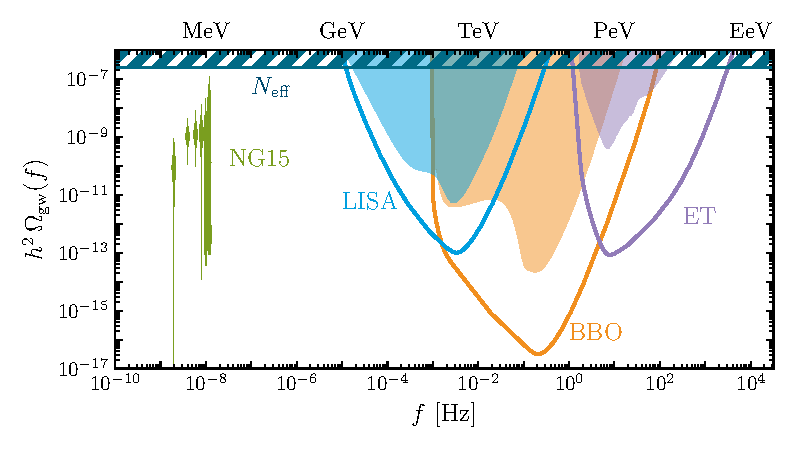
\includegraphics[width=\linewidth]{thesisplots/observability/observability.pdf}
	\caption{Overview of observational bounds on primordial \acp{GWB}. The blue, orange and purple filled areas correspond to the expected effective noise spectra $h^2\Omega_\text{eff}$ of the interferometers \ac{LISA}, \ac{BBO} and \ac{ET} from ref.~\cite{Breitbach:2018ddu}. The dips in the spectra correspond to the expected unresolved astrophysical background from galactic and extra-galactic white dwarf binaries. The blue, orange and purple contours are the associated \acs{PLI} curves. The green violins depict the six lowest Fourier modes of the free-spectral analysis of the \ac{NANOGrav} 15yr data set. The blue hatched band corresponds to the \Neff bound on primordial \acp{GWB} from eq.~\eqref{eq:NeffboundGW}.}
	\label{fig:observability}
\end{figure}

Given an effective noise spectrum $\Omega_\text{eff}(f)$ of an \graffito{The SNR of an interferometer} observatory, which is understood to include all relevant noise contributions from the detector but also from unresolved astrophysical backgrounds, we can construct the optimal-filter cross-correlated \ac{SNR} for a cosmological \ac{GWB}
\begin{align}
	\rho^2 = 2 \, t_\text{obs} \int_{f_\text{min}}^{f_\text{max}} \diff f\, \bb{\frac{ \Omega_\gw(f)}
		{\Omega_\text{eff}(f)} }^2 \, .
	\label{eq:SNR}
\end{align}
The factor $t_\text{obs}$ denotes the duration of the observation and the observatory's frequency band spans $f_\text{min}$ to $f_\text{max}$. The initial factor of 2 only appears when the \ac{SNR} refers to a cross-correlation between different detectors. If instead an auto-correlation is used by the observatory, this factor 2 drops out of the equation. We will refer to a \ac{GW} signal as observable if its \ac{SNR} exceeds a given specific threshold, $\rho \ge \rho_\text{thr}$, which we list in table~\ref{tab:detectors}.

\begin{table}
	\centering
	\begin{tabular}{lcccc}
		\toprule
		Experiment      &               Frequency range               &    $\SNR_\text{thr}$    &  $t_\text{obs}$   & Auto-correlated? \\ \hline
		\acs{LISA}            & $\SI{e-5}{}-\SI{1}{Hz}$ & $10$& $4 \, \text{yrs}$ & \cmark                          \\
		\acs{BBO}             & $\SI{e-3}{}-\SI{e2}{Hz}$ &          $10$           & $4 \, \text{yrs}$ & \xmark                           \\
		\acs{ET}              &  $\SI{1}{}-\SI{e4}{Hz}$  & $5$  & $5 \, \text{yrs}$ & \cmark                          \\ \bottomrule
	\end{tabular}
	\caption{Threshold \acsp{SNR} $\rho_\text{thr}$ of future \ac{GW} observatories taken from ref.~\cite{Breitbach:2018ddu}.}
	\label{tab:detectors}
\end{table}

If $\Omega_\gw(f)$ follows a power-law, it \graffito{PLI curves} is convenient to not show $\Omega_\text{eff}(f)$ in plots as a comparison, but instead use so-called \ac{PLI} curves $\Omega_\text{PLI}(f)$. For a given observatory, they are defined as 
\begin{align}
		\Omega_\text{PLI}(f) = \max \limits_b \bb{\Omega_b^\text{thr}
		\ba{\frac{f}{\bar{f}}}^b} \,,
\end{align}
where $\bar{f}$ is an arbitrary pivot frequency and
\begin{align}
	\Omega_b^\text{thr} \equiv \frac{\rho_\text{thr}}{\sqrt{2\, t_\text{obs}}} \bb{ \int_{f_\text{min}}^{f_\text{max}} \diff f \,
		\ba{ \frac{\ba{f/\bar{f}}^b}{\Omega_\text{eff}(f)} }^2}^{-\frac{1}{2}} 
\end{align}
is the minimum signal amplitude needed in order to reach the observatory's \ac{SNR} threshold $\rho_\text{thr}$ for a  power-law shaped \ac{GWB} $\Omega_\gw(f) =  \Omega_b \ba{\frac{f}{\bar{f}}}^b$. If a given power-law shaped \ac{GWB} spectrum intersects with the \ac{PLI} spectrum, it can be considered observable by the respective observatory. However, it’s important to note that this interpretation is only indicative if the signal does not actually follow a power-law shape. In such cases, comparing the \ac{SNR} from eq.~\eqref{eq:SNR} with the threshold value provided in table~\ref{tab:detectors} is necessary to reach a definitive conclusion.

Fig.~\ref{fig:observability} also shows the so-called Bayesian spectrograms (commonly referred to as violins) for the \ac{NANOGrav} 15yr data set. We will discuss the \graffito{A note on violins} precise origin and interpretation of these in detail in chapter \ref{chp:PTAs}. An easy way of interpreting them is as data points whose error bars have been upgraded to a full statistical distribution which is depicted as the violin's width. Note, however, that this interpretation can be misleading as it forgets about the Bayesian character of these distributions: The vanishing width of a given violin at low signal amplitudes does not indicate that it is impossible for the signal to have an amplitude lower than indicated by the violins. Instead, the range of the violins rather indicates the boundaries of their underlying prior ranges.

In fig.~\ref{fig:observability} we also show $\DNeff$ bounds on primordial \acp{GWB}. In section~\ref{sec:BBN} \graffito{The $N_\mathrm{eff}$ bound on primordial \acp{GWB}} we introduced the quantity $\DNeff$ which parameterizes any additional energy density $\rho_\text{extra}$ in units of neutrino \acp{dof} after their decoupling. Both \ac{BBN} and the \ac{CMB} observables can be used to infer bounds on the Hubble rate around the temperature of neutrino decoupling and recombination, which can then be expressed in terms of bounds on $\DNeff$. If one equates the energy density $\rho_\text{extra}$ in eq.~\eqref{eq:DNeff} with the energy density $\rho_\gw$ of a primordial \ac{GWB}, one can obtain a bound on its amplitude.

Using as reference values the 95\% C.L. upper limit on \Neff from \ac{BBN} and \ac{CMB} combined from eq.~\eqref{eq:BBNCMBNeff}~\cite{Yeh:2022heq}, $\Neff = 2.941 + 0.143 = 3.084$, and the corresponding $\DNeff = 3.084-3.044 = 0.040$ as a normalization, we obtain  
\begin{align}
	\left. \frac{\rho_\gw}{ \rho_\gamma} \right|_{t_\text{BBN}} = \left. \frac{\rho_\gw}{ \rho_\gamma} \right|_{t_0} < 9.1 \cdot 10^{-3} \ba{\frac{N_{\text{eff}}-3.044}{0.040}} .
\end{align}
To arrive at this conclusion we used that after the $e^{+} e^{-}$-annihilation the photon energy density redshifts precisely like the \ac{GW} energy density until today. Of course, this bound can only depend on the energy density of a primordial signal produced before $T \sim 0.1 \, \text{MeV}$, corresponding to the onset of \ac{BBN} after the deuterium bottleneck. In particular,  \graffito{$N_\mathrm{eff}$ puts bounds on the integrated spectrum} astrophysical backgrounds are therefore not affected by this bound. It should further be noted, that this bound can only depend on modes that already entered the Hubble sphere at that time. This corresponds to \acp{GW} which today have frequencies above $f_\text{BBN} \simeq 1.5 \cdot 10^{-11} \, \text{Hz}$. To arrive at this value we used eq.~\eqref{eq:fredshiftsimple} and for definiteness put in $x_k = 10$, requiring that only modes well within the Hubble sphere contribute. Using $h^2 \Omega_\gamma= 2.473 \cdot 10^{-5}$, we can equivalently write
\begin{align}
	\int_{f_{\text{BBN}}}^{\infty} \frac{\diff f}{f} \,  h^2 \Omega_\gw(f)<2.5 \times 10^{-7} \ba{\frac{\Neff-3.044}{0.040}}.
\end{align}
If we further assume that the signal is peaked  over at least an order of magnitude in frequency (which is typically the case), we can further impose
\begin{align}
	h^2 \Omega_{\gw}(f) \lesssim 2.5 \times 10^{-7} \ba{\frac{\Neff-3.044}{0.040}} \quad \text{for} \quad f>f_\text{BBN} \, , \label{eq:NeffboundGW}
\end{align}
which is the \ac{BBN} bound shown in fig.~\ref{fig:observability}. 

There are considerable ongoing  \graffito{No sensitivity to primordial \acp{GW} at high frequencies} efforts to extend the probed \ac{GW} spectrum to higher frequencies~\cite{Bringmann:2023gba, Berlin:2023grv}.  These proposals for instance recommend the use of the inverse Gertsenshtein effect, i.e.~the coupling of \acp{GW} to electromagnetic fields, or the direct mechanical coupling of radio frequency cavities to \acp{GW} for their detection. So far, the existing limits are far from exceeding the $\DNeff$ bound. We therefore do not show any further bounds at higher frequencies.

The upper horizontal axis in fig.~\ref{fig:observability} corresponds to the temperature $T_*$ a given frequency refers to according to eq.~\eqref{eq:fredshiftsimple}, where we set $x_k = 1$ for definiteness and ignored the mild dependence of $g_* \simeq \mathcal{O}(100)$ on temperature. It hence becomes apparent that the \ac{PTA} signal hints towards strong dynamics in the primordial plasma at MeV temperatures, \graffito{We live in the age of \ac{GW} cosmology!} whereas \ac{GW} observatories sensitive to higher frequencies will be able to probe the primordial plasma at even higher temperatures. Previously, \ac{BBN} was considered the earliest direct probe of the \ac{LCDM} model. With the advancement of sensitivities for \acp{GWB} at higher frequencies, we will therefore be able to directly probe the occurrence of anisotropic stress in the primordial plasma at much earlier times. We can thus rightfully claim: we are at the the dawn of \ac{GW} cosmology!